\documentclass[sigconf,screen]{acmart} 


% to be able to draw some self-contained figs
\usepackage{tikz}
\usepackage{amsmath}
% \usepackage{amssymb}
\usepackage{multirow}
\usepackage{makecell}
% inlined bib file
% \usepackage{filecontents}
\usepackage{enumitem}

% -------------------------------------------------------------------------------
% PARASAIL TEAM PACKAGES
%-------------------------------------------------------------------------------
%% Some recommended packages.
\usepackage{booktabs}   %% For formal tables:
                        %% http://ctan.org/pkg/booktabs
\usepackage{subcaption} %% For complex figures with subfigures/subcaptions
                        %% http://ctan.org/pkg/subcaption
\captionsetup{compatibility=false}

\newcommand{\asplossubmissionnumber}{1601}

\usepackage[normalem]{ulem}
\usepackage{xspace}
\usepackage{color}
\usepackage{listings}
\usepackage{tikz}
\usepackage{listings}
\usepackage{graphicx}
\usepackage{mathpartir}
\usepackage{float}
\usepackage{textcomp}
\usepackage{pythonhighlight}
\usepackage{algorithm}
\usepackage{tabularx}
\usepackage{algpseudocode}% http://ctan.org/pkg/al
\usepackage{pervasives}
\usepackage{balance}

%%% If you see 'ACMUNKNOWN' in the 'setcopyright' statement below,
%%% please first submit your publishing-rights agreement with ACM (follow link on submission page).
%%% Then please update our instructions page and copy-and-paste the NEW commands into your article.
%%% Please contact us in case of questions; allow up to 10 min for the system to propagate the information.
%%%
%%% The following is specific to ASPLOS '22 and the paper
%%% 'Breaking the Computation and Communication Abstraction Barrier in Distributed Machine Learning Workloads'
%%% by Abhinav Jangda, Jun Huang, Guodong Liu, Amir Hossein Nodehi Sabet, Madan Musuvathi, Olli Saarikivi, Saeed Maleki, Todd Mytkowicz, and Youshan Miao.
%%%
% \setcopyright{ACMUNKNOWN}
%setcopyright before submission (https://www.conference-publishing.com/Instructions.php?Event=ASPLOS22MAIN&Paper=dc7505a434aecf501da1e25d14ec02d294b684e8)

%%% The following is specific to ASPLOS '22 and the paper
%%% 'Breaking the Computation and Communication Abstraction Barrier in Distributed Machine Learning Workloads'
%%% by Abhinav Jangda, Jun Huang, Guodong Liu, Amir Hossein Nodehi Sabet, Saeed Maleki, Youshan Miao, Madan Musuvathi, Todd Mytkowicz, and Olli Saarikivi.
%%%
\setcopyright{acmcopyright}
\acmPrice{15.00}
\acmDOI{10.1145/3503222.3507778}
\acmYear{2022}
\copyrightyear{2022}
\acmSubmissionID{asplos22main-p1601-p}
\acmISBN{978-1-4503-9205-1/22/02}
\acmConference[ASPLOS '22]{Proceedings of the 27th ACM International Conference on Architectural Support for Programming Languages and Operating Systems}{February 28 -- March 4, 2022}{Lausanne, Switzerland}
\acmBooktitle{Proceedings of the 27th ACM International Conference on Architectural Support for Programming Languages and Operating Systems (ASPLOS '22), February 28 -- March 4, 2022, Lausanne, Switzerland}


%-------------------------------------------------------------------------------
\begin{document}
%-------------------------------------------------------------------------------

%don't want date printed
\date{}

% make title bold and 14 pt font (Latex default is non-bold, 16 pt)
% \title{\tool: Co-Optimizing Computation and Communication for Distributed Machine Learning}
\title[Breaking the Computation and Communication Abstraction Barrier in Distributed ML Workloads]{Breaking the Computation and Communication Abstraction Barrier in Distributed Machine Learning Workloads}
%\title{Bridging the Computation-Communication Abstraction \\ to Co-optimize Distributed Machine Learning}

\author{Abhinav Jangda}
\affiliation{
    \institution{University of Massachusetts Amherst}
    \country{United States}
}
\author{Jun Huang}
\affiliation{
    \institution{Ohio State University}
    \country{United States}
}
\author{Guodong Liu}
\affiliation{
    \institution{Chinese Academy of Sciences}
    \country{China}
}
\author{Amir Hossein Nodehi Sabet}
\affiliation{%
  \institution{University of California, Riverside}
  \country{United States}
}
\author{Saeed Maleki}
\affiliation{%
  \institution{Microsoft Research}
  \country{United States}
}
\author{Youshan Miao}
\affiliation{%
  \institution{Microsoft Research}
  \country{China}
}
\author{Madanlal Musuvathi}
\affiliation{%
  \institution{Microsoft Research}
  \country{United States}
}
\author{Todd Mytkowicz}
\affiliation{%
  \institution{Microsoft Research}
  \country{United States}
}
\author{Olli Saarikivi}
\affiliation{%
  \institution{Microsoft Research}
  \country{United States}
}

\renewcommand{\shortauthors}{A. Jangda, J. Huang, G. Liu, A. H. N. Sabet, S. Maleki, Y. Miao, M. Musuvathi, T. Mytkowicz, O. Sarikivi}


% % %for single author (just remove % characters)
% \author{
% {\rm Abhinav Jangda}\\
% University of Massachusetts Amherst
% \and
% {\rm Jun Huang}\\
% Ohio State University
% \and
% {\rm Guodong Liu}\\
% Chinese Academy of Sciences
% \and
% {\rm Amir Hossein Nodehi Sabet}\\
% University of California, Riverside
% \and
% {\rm Madan Musuvathi}\\
% Microsoft Research
% \and
% {\rm Olli Saarikivi}\\
% Microsoft Research
% \and
% {\rm Saeed Maleki}\\
% Microsoft Research
% \and
% {\rm Todd Mytkowicz}\\
% Microsoft Research
% \and
% {\rm Youshan Miao}\\
% Microsoft Research
% } % end author

%-------------------------------------------------------------------------------
\begin{abstract}
Recent trends towards large machine learning models require both training and inference tasks to be distributed.
Considering the huge cost of training these models, it is imperative to unlock optimizations in computation and communication to obtain best performance.
However, the current logical separation between computation and communication kernels in machine learning
frameworks misses optimization opportunities across this barrier.
Breaking this abstraction can provide many optimizations to improve the performance 
of distributed workloads.
However, manually applying these optimizations requires modifying the underlying computation and communication libraries for each scenario, which is both time consuming and error-prone.

Therefore, we present \tool{}, which 
contains (i) a domain specific language to express a distributed machine learning program in the form of computation and communication operations, (ii) a set of semantics preserving transformations to optimize the program, and (iii) a compiler to generate jointly optimized communication and computation GPU kernels.
Providing both computation and communication as first class constructs allows users to work on a high-level abstraction and
apply powerful optimizations, such as fusion or overlapping of communication and computation.
\tool 
enabled us to optimize data-, model- and pipeline-parallel workloads in large language models with only a few lines of code. 
Our experiments show that \tool 
significantly outperforms state-of-the-art distributed machine learning implementations.
\end{abstract}
\begin{CCSXML}
<ccs2012>
<concept>
<concept_id>10011007.10011006.10011050.10011017</concept_id>
<concept_desc>Software and its engineering~Domain specific languages</concept_desc>
<concept_significance>500</concept_significance>
</concept>
<concept>
<concept_id>10011007.10011006.10011041</concept_id>
<concept_desc>Software and its engineering~Compilers</concept_desc>
<concept_significance>500</concept_significance>
</concept>
<concept>
<concept_id>10010147.10010169</concept_id>
<concept_desc>Computing methodologies~Parallel computing methodologies</concept_desc>
<concept_significance>500</concept_significance>
</concept>
</ccs2012>
\end{CCSXML}

\ccsdesc[500]{Software and its engineering~Domain specific languages}
\ccsdesc[500]{Software and its engineering~Compilers}
\ccsdesc[500]{Computing methodologies~Parallel computing methodologies}

\keywords{Distributed Machine Learning, Collective Communication, MPI, CUDA, Code Generation, Compiler Optimizations}

\maketitle


% \settopmatter{printfolios=true}
%\settopmatter{printacmref=false} % Removes citation information below abstract


% \pagestyle{plain} % removes running headers


\section{Introduction}
Despite the well-recognized importance of training data in advancing the capabilities of large language models (LLMs)~\cite{brown2020language,kaplan2020scaling,Razeghi2022ImpactOP}, there is no agreed-upon mechanisms for crediting or compensating data providers. As LLMs are increasingly integrated into our society and economy, the absence of such mechanisms has aggravated a tension between data and model providers, exemplified by recent legal challenges involving major tech companies~\cite{jlversusalphabet,metz2022lawsuit}. In this atmosphere, data valuation, which quantifies the contribution of each training data to the model output, has been discussed as a potential technical solution for tackling these societal issues~\cite{fernandez2023data,ghorbani2019data,huang2023citation,jia2019towards,worledge2023unifying,zhao2023addressing}. 

At a high level, most data valuation algorithms interpret the model output as a coalition of its training data, and evaluate the contribution of each example based on its influence on the model output when included or excluded from the training dataset~\cite{ghorbani2019data,ilyas2022datamodels,koh2017understanding,kwon2021beta}. If an inclusion of a specific training example consistently improves model performance, high value can be assigned to this example for its contribution. However, applying existing data valuation methods to recent LLMs and their vast training datasets has faced significant scalability challenges to date. For instance, sampling-based methods, such as the Shapley value~\cite{ghorbani2019data,kwon2021beta} or Datamodels~\cite{ilyas2022datamodels}, require retraining the model multiple times with varied combinations of data subsets to directly model the effect of in/excluding each data. Unfortunately, such repeated retraining is hardly affordable even for small models, let alone LLMs. To overcome this issue, gradient-based methods, including influence functions~\cite{koh2017understanding,park2023trak}, approximate the effect of data in/exclusion on the model output using gradient information without costly retraining. Even so, scaling gradient-based methods to LLMs is hindered by prohibitive compute and memory costs originating in the high-dimensional nature of the gradient.

Consequently, the main objective of this work is to bridge the gap in scaling existing data valuation methods to recent LLMs and their vast training datasets. Toward this goal, we focus on influence functions \cite{koh2017understanding,park2023trak}, a representative gradient-based data valuation method, and significantly improve its scalability with an efficient gradient projection algorithm. We visualize the proposed data valuation system in Figure~\ref{fig:diagram}, and detail our technical contributions below:

\begin{figure}
    \centering
    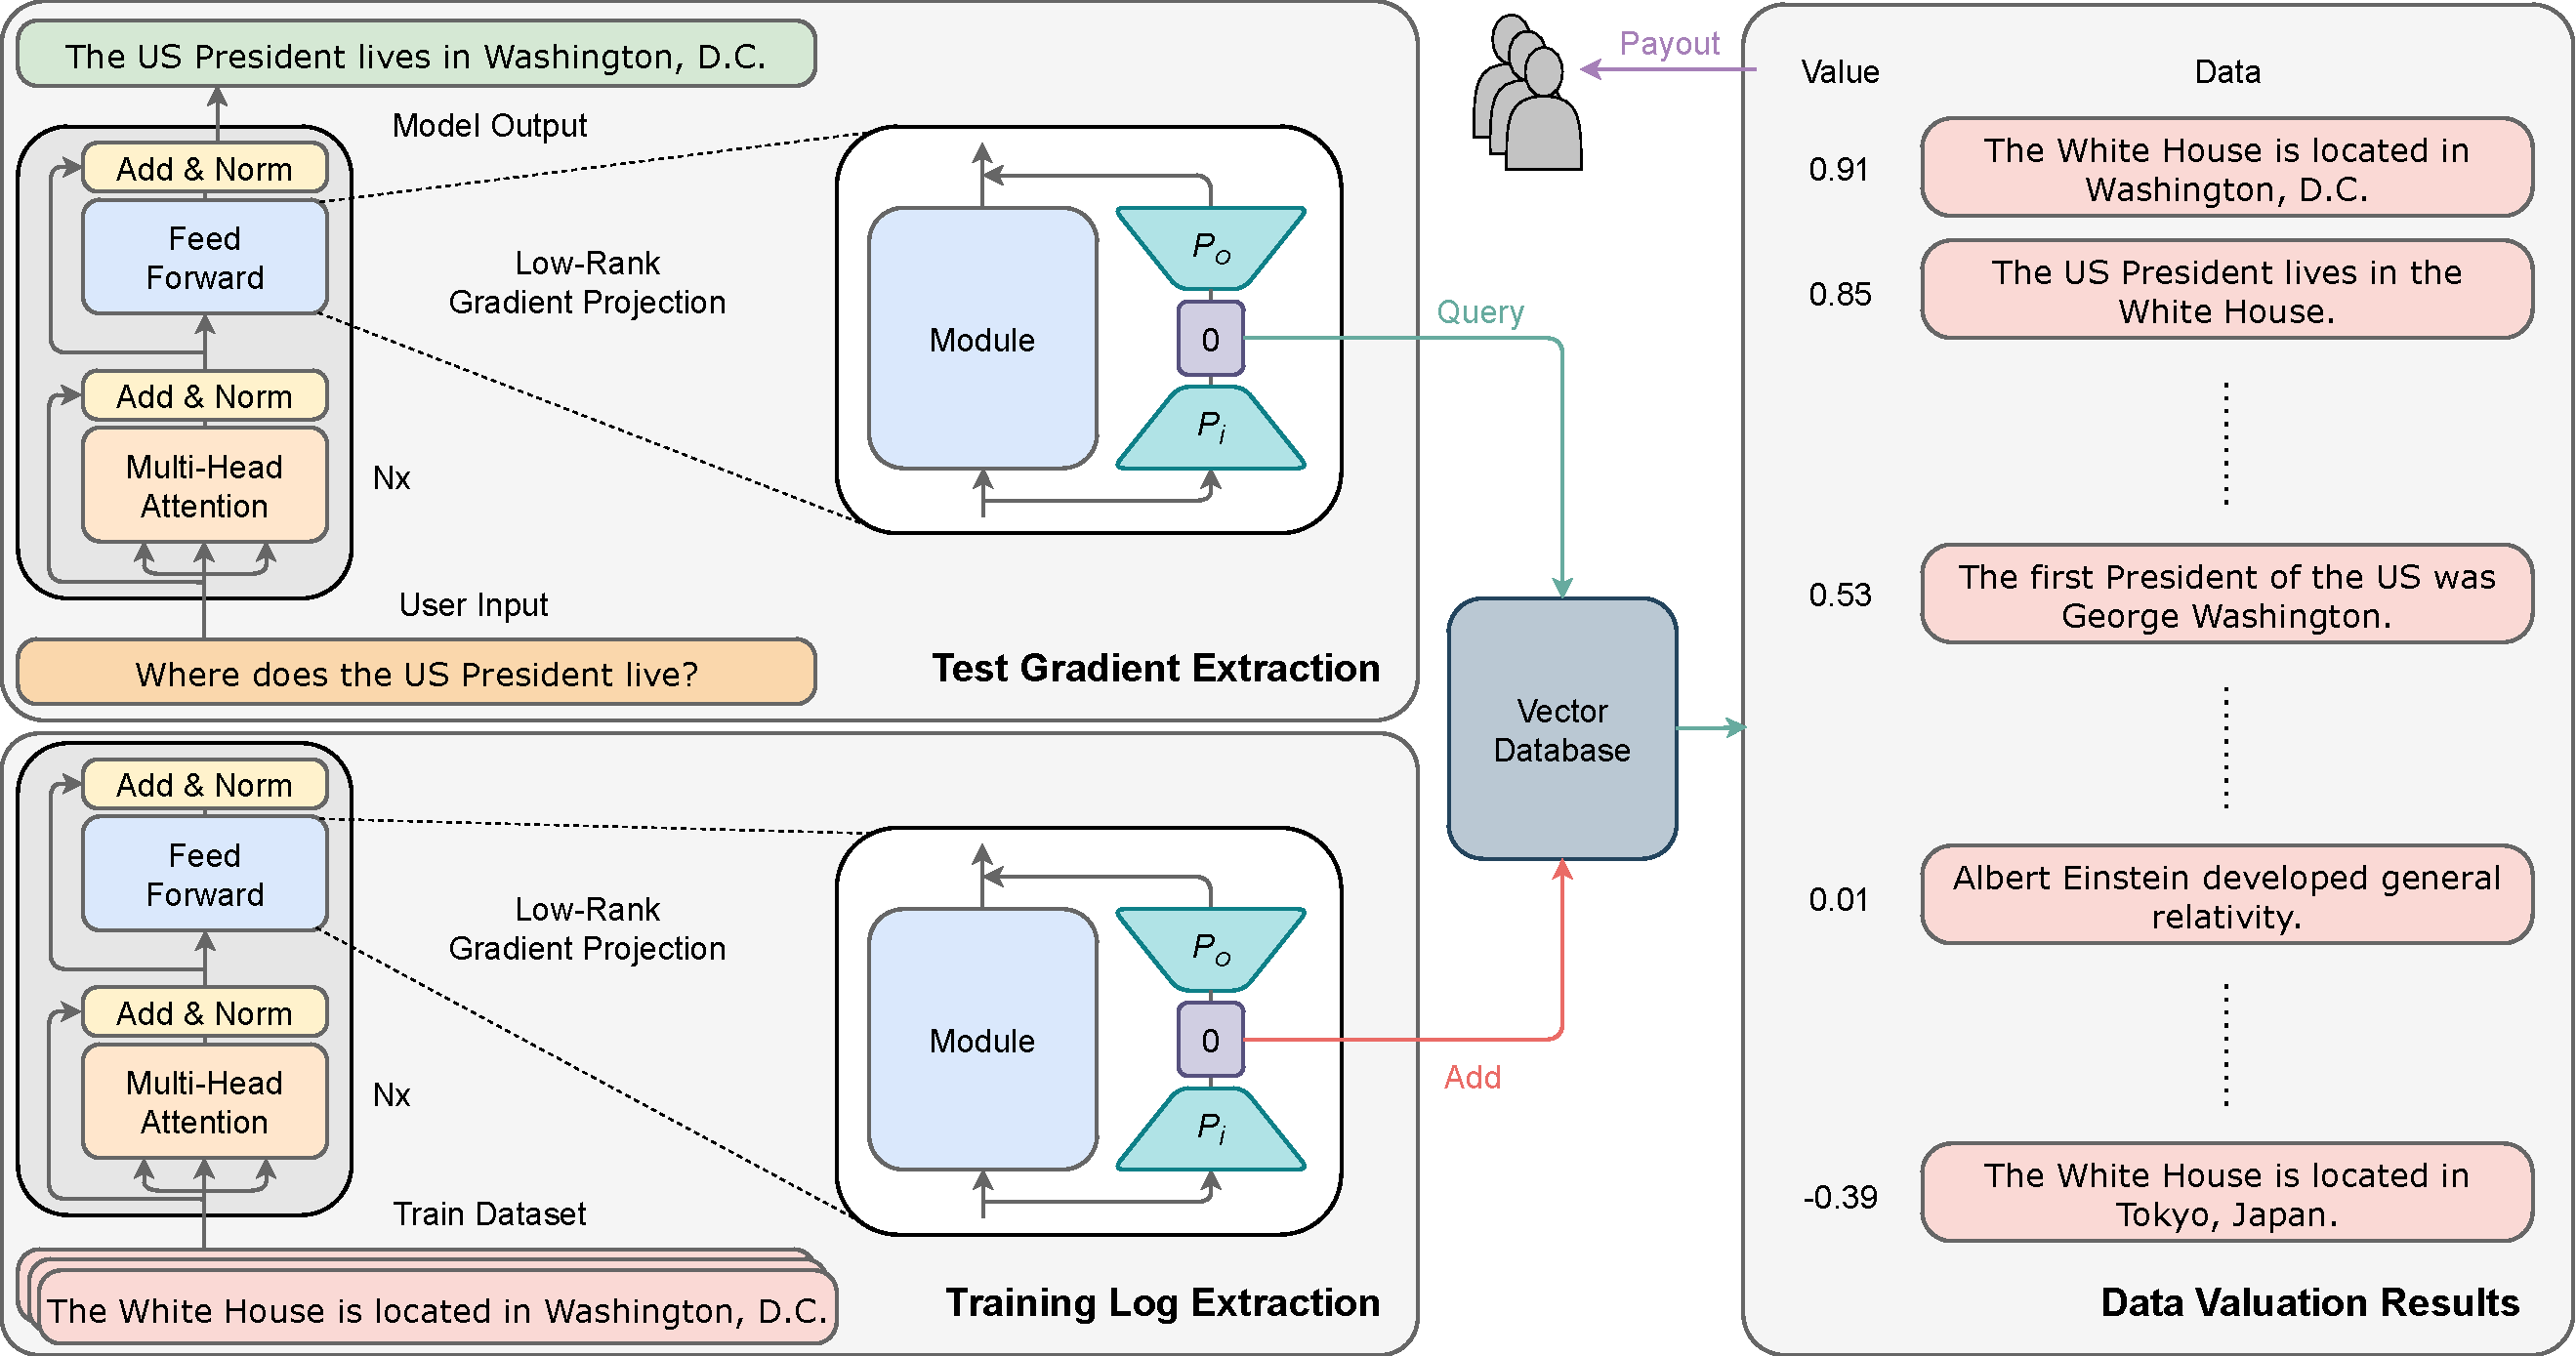
\includegraphics[width=0.94\textwidth]{figures/diagram_v7.pdf}
    \vskip -4pt
    \caption{Data valuation system architecture. \textbf{(Left Bottom)} We first extract the Hessian and gradients for all training data using efficient gradient projection \method\ and store them in a database. \textbf{(Left Top)} At test time, we similarly extract gradients and query the database. \textbf{(Right)} The database returns similarity scores with respect to training examples that can be used for data valuation/attribution.}
    \label{fig:diagram}
\end{figure}

\begin{itemize}[leftmargin=*,topsep=-2pt]
    \item Employing gradient structures in backpropagation, we develop a novel \textbf{lo}w-rank \textbf{gra}dient projection algorithm \method\ that improves space \& time complexity of gradient projection, a major scalability bottleneck in prior work~\cite{park2023trak,schioppa2022scaling}, from $O(nk)$ to $O(\sqrt{nk})$ where $n$ and $k$ are model and projection dimensions. Furthermore, \method\ directly computes projected gradients without materializing full gradients, enabling low GPU memory and high GPU utilization for improved efficiency. Lastly, we show that \method\ can be easily implemented with small add-on layers, similarly to LoRA~\cite{hu2021lora}.
    \item By interpreting a damping term in influence functions as a spectral gradient sparsification mechanism, we (1) offer a theoretical motivation of gradient projection approaches to influence functions and (2) derive a specialized PCA initialization scheme for \method.
    \item We introduce software named \software\ that (1) makes it \textit{simple} to convert existing training code into data valuation code, (2) is \textit{compatible} with various scalability tools and features in the LLM ecosystem, and (3) is \textit{extensible} to implement other data valuation or interpretability algorithms.
    \item In our data valuation experiments, \method\ demonstrates competitive accuracy against more costly baselines, while showing up to 6,500$\times$ increase in throughput and 5$\times$ reduction in GPU memory, when applied to Llama3-8B-Instruct~\cite{llama3modelcard} and the 1B-token dataset, compared to EKFAC influence \cite{grosse2023studying}, the state-of-the-art and only runnable baseline at this scale. We also observe that most valuable data identified by \method\ generally share qualitative similarities with the queried LLM output.
\end{itemize}
%\subsection{Data Augmentation in NLP}
The problem of domain adaptation and OOD robustness is well established in NLP \citep{blitzer-etal-2007-biographies,daume-iii-2007-frustratingly,hendrycks2020pretrained}.
Existing work on improving generalization has focused on data augmentation, where synthetically generated training examples are used to augment an existing dataset.
It is hypothesized that these examples induce robustness to local perturbations, which has been shown to be effective in semi-supervised and self-supervised settings \citep{bachman2014learning,szegedy2014intriguing, sajjadi2016regularization}.

Existing task-specific methods \citep{kafle-etal-2017-data} and word-level methods \citep{zhang2015character, xie2017data, wei-zou-2019-eda} are based on human-designed heuristics.
Back-translation from or through another language has been applied in the context of machine translation \citep{sennrich2016improving}, question answering \citep{wei2018fast}, and consistency training \citep{xie2019unsupervised}.
More recent work has used word embeddings \citep{wangyang2015thats} and LSTM language models \citep{fadaee2017data} to perform word replacement.
Other methods focus on fine-tuning contextual language models \citep{kobayashi-2018-contextual,wu2019conditional,kumar20202data} or large generative models \citep{lambada,yang2020g-daug,kumar20202data} to generate synthetic examples.

\subsection{VRM and the Manifold Assumption}
Vicinal Risk Minimization (VRM) \citep{vicinal200olivier} formalizes data augmentation as enlarging the training set support by drawing samples from a \textit{vicinity} of existing training examples.
Typically the vicinity of a training example is defined using dataset-dependent heuristics.
For example, in computer vision, examples are generated using scale augmentation \citep{simonyan2014very}, color augmentation \citep{krizhevsky2012imagenet}, and translation and rotation \citep{Simard1998}.

The \textit{manifold assumption} states that high dimensional data concentrates around a low-dimensional manifold \citep{chapelle2006semi}.
This assumption allows us to define the vicinity of a training example as its \textit{manifold neighborhood}, the portion of the neighborhood that lies on the data manifold.
Recent methods have used the manifold assumption to improve robustness by moving examples towards a decision boundary \citep{kanbak2018geometric}, generating adversarial examples \cite{szegedy2014intriguing,miyato2017virtual}, interpolating between pairs of examples \citep{zhang2018mixup}, or finding affine transforms \citep{paschali2019data}.

\begin{figure}[t!]
\centering
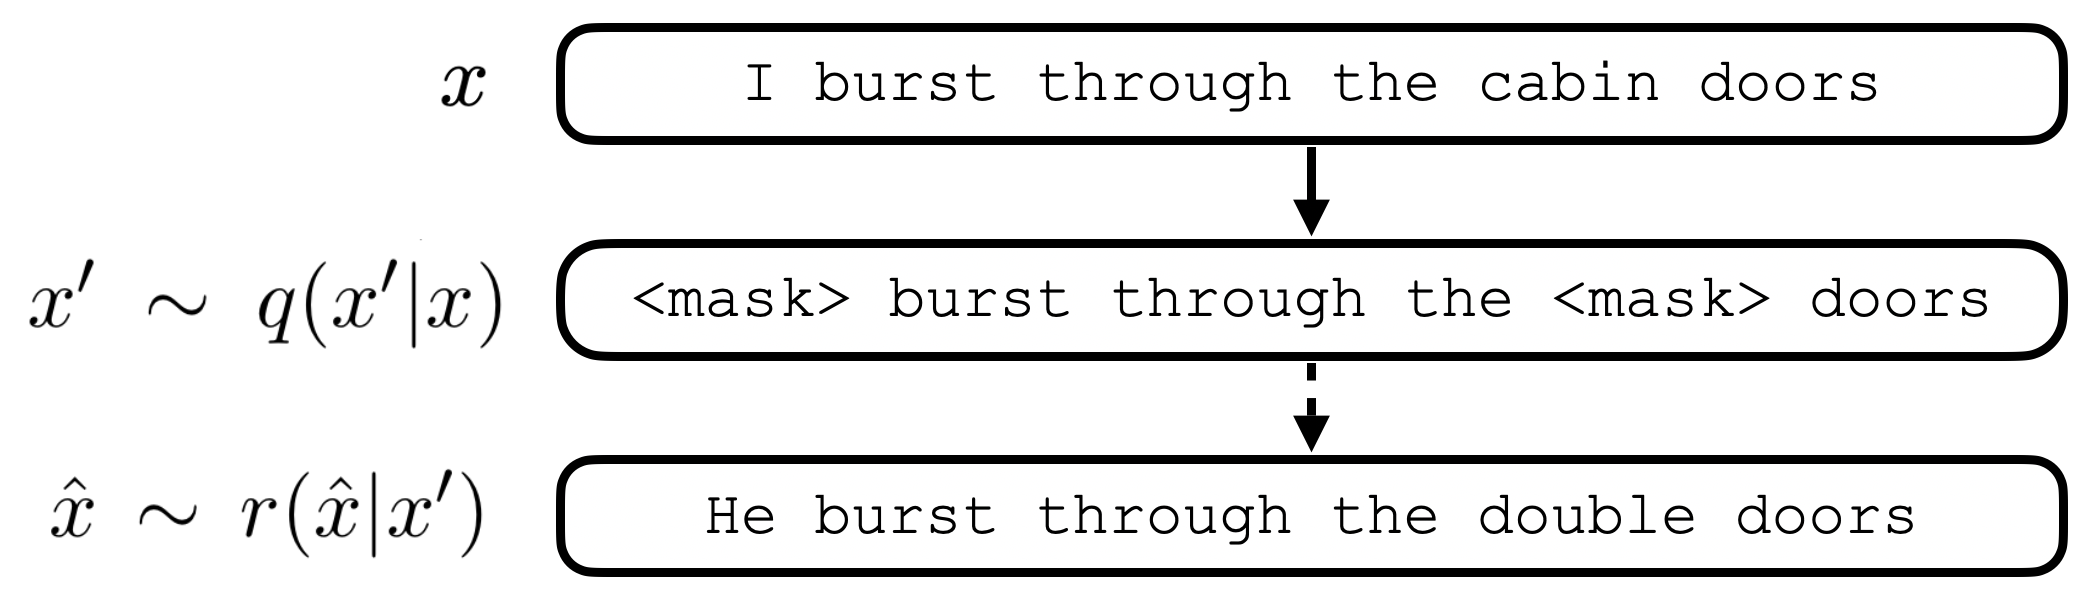
\includegraphics[scale=0.21]{img/bert_dae.png}
\caption{To sample from an MLM DAE, we apply the MLM corruption $q$ to the original sentence then reconstruct the corrupted sentence using our DAE $r$.}
\label{fig:dae_sampling}
\end{figure}

\subsection{Sampling from Denoising Autoencoders}
A denoising autoencoder (DAE) is an autoencoder trained to reconstruct a clean input $x$ from a stochastically corrupted one $x'\sim q(x'|x)$ by learning a conditional distribution $P_\theta (x| x')$ \citep{vincent2008extracting}.
We can sample from a DAE by successively corrupting and reconstructing an input using the following pseudo-Gibbs Markov chain: $x_t' \sim q(x'|x_{t-1})$, $x_t \sim P_\theta(x|x'_t).$
\comment{
\begin{align*}
    x_t' &\sim q(x'|x_{t-1})\\
    x_t &\sim P_\theta(x|x'_t) 
\end{align*}
}
As the number of training examples increases, the asymptotic distribution $\pi_n(x)$ of the generated samples approximate the true data-generating distribution $P(x)$ \citep{bengio2013generalized}.
This corruption-reconstruction process allows for sampling directly along the manifold that $P(x)$ concentrates on.

\subsection{Masked Language Models}
Recent advances in unsupervised representation learning for natural language have relied on pre-training models on a \textit{masked language modeling} (MLM) objective \citep{devlin2018, liu2019roberta}.
In the MLM objective, a percentage of the input tokens are randomly corrupted and the model is asked to reconstruct the original token given its left and right context in the corrupted sentence.
We use MLMs as DAEs \citep{lewis2019bart} to sample from the underlying natural language distribution by corrupting and reconstructing inputs (Figure \ref{fig:dae_sampling}).

%\section{Motivation}

% \section{Fused Communication Collectives}
In this section, we describe bla bla bla \aj{TODO}

All communication collectives provided by NCCL can be conceptually described using a series of three primitives: (i) \texttt{SEND} that sends data from one rank to other, (ii) \texttt{RECV} that receives data from another rank, and (iii) \texttt{REDUCE} that performs reduction based on a reduction operator.
For example, in \reduce each rank first \texttt{SEND}s data, then the destination rank \texttt{RECV}s data, and finally the destination rank performs \texttt{REDUCE} on the data received.
In distributed model training, it is common that pointwise computations are performed on the data received after communication collectives, or the input to communication collectives are output of a pointwise computations.
For example, in synchronous Adam the average of all gradients distributed among different ranks is obtained using \allreduce and several pointwise computations are performed to do parameter update.
Existing techniques writes the output of communication collectives to a memory location, loads from that location and performs the computation.
Hence, this requires one store for storing the output and one load for loading the output.

However, we can remove these extra stores and loads by fusing the pointwise computations with any of the primitives, thereby passing the results of communication collectives to the computation from registers instead.
For example, 

\begin{table*}
  \small
  % \begin{subtable}{\textwidth}
    \begin{tabular}[]{|l|l|l|l|l|}\hline
      \thead{Computation with\\ Communication Collective} & Series of Primitives & Fused Communication Collective\\ \hline
      $f_2($\reduce($f_1(t)$,redOp)) & $f_1(t)\rightarrow$ SEND $\rightarrow$ RECV $\rightarrow$ $f_2$(REDUCE(redOp)) & FusedReduce(t, $f_1$, redOp, $f_2$)\\ \hline
      $f_2($\broadcast($f_1(t)$)) & $f_1(t)\rightarrow$ SEND $\rightarrow$ $f_2$(RECV) & FusedBroadcast(t, $f_1$, $f_2$)\\ \hline
      $f_2($\allreduce($f_1(t)$,redOp)) & \thead{$f_1(t)\rightarrow$SEND $\rightarrow$ RECV $\rightarrow$ $f_2$(REDUCE(redOp)) \\$\rightarrow$ SEND $\rightarrow$ RECV} & FusedAllReduce(t, $f_1$, redOp, $f_2$)\\ \hline
      $f_2($\reducescatter($f_1(t)$,redOp)) &  $f_1(t)\rightarrow$ SEND $\rightarrow$ RECV $\rightarrow$ $f_2$(REDUCE(redOp)) & FusedReduceScatter(t, $f_1$, redOp, $f_2$) \\ \hline
      $f_2($\allgather($f_1(t)$)) & $f_1(t)\rightarrow$SEND $\rightarrow$ $f_1$(RECV) & FusedAllGather(t, $f_1$, $f_2$)\\ \hline

    \end{tabular}

  \caption{Computation over Communication Collectives can be described in a series of SEND, RECV, and REDUCE primitives. We formalize these primitives into Fused Communication Collectives.}
\end{table*}


% \begin{figure*}[t]
    \centering
    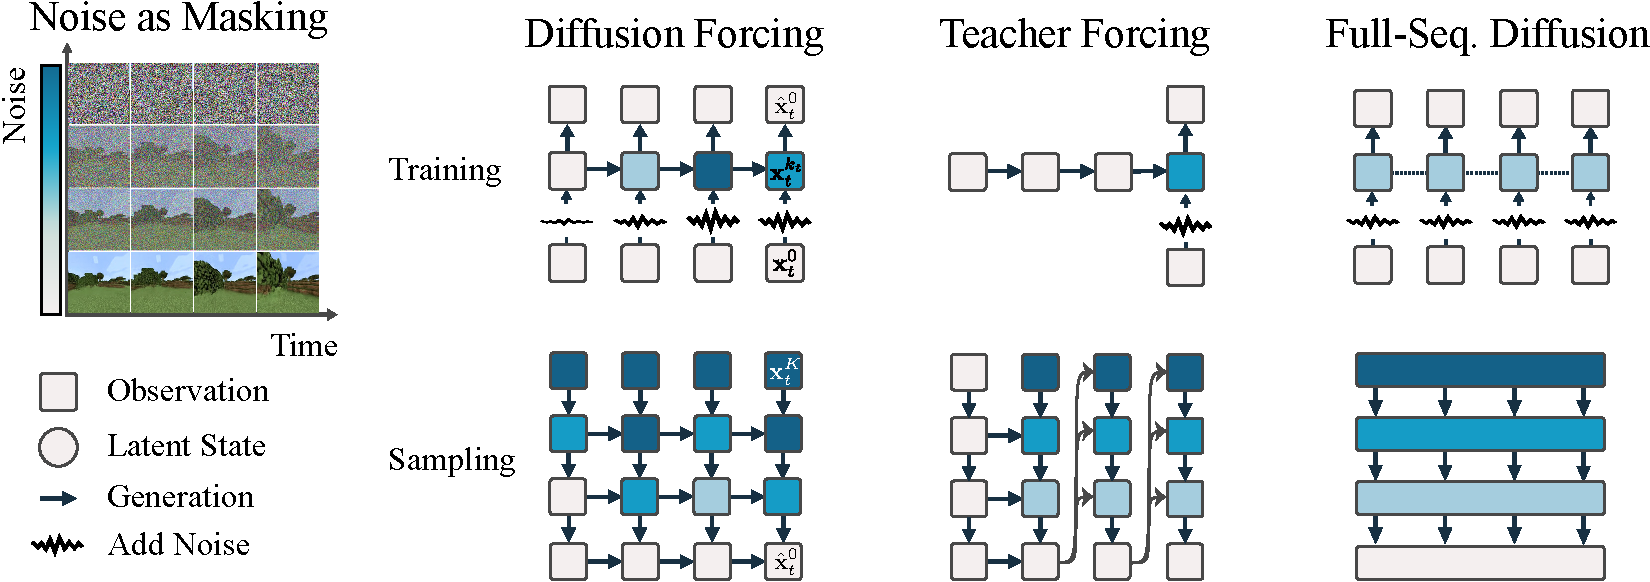
\includegraphics[width=\linewidth]{figures/pdf/Overview_best_guess.pdf}
    \caption{\textbf{Method Overview.} 
    Diffusion Forcing trains causal sequence neural networks (such as an RNN or a masked transformer) to denoise flexible-length sequences where each frame of the sequence can have a \emph{different} noise level.
    In contrast, next-token prediction models, common in language modeling, are trained to predict a single next token from a \emph{ground-truth} sequence (teacher forcing~\cite{teacher_forcing}), and full-sequence diffusion, common in video generation, train non-causal architectures to denoise all frames in a sequence at once with the \emph{same} noise level.
    \algo{} thus \emph{interleaves} the time axis of the sequence and the noise axis of diffusion, unifying strengths of both alternatives and enabling completely new capabilities (see Secs.~\ref{sec:zigzag_example},\ref{sec:method_decision_making}).
    }
    \label{fig:method}
    \vspace{-5pt}
\end{figure*}
 %Overview has been integrated in the introduction
\section{The \tool DSL}
\label{sec:dsl}
The \tool DSL extends the data representation in existing machine learning frameworks and provides constructs to express both computation and communication. 
The \tool DSL is embedded in C++.
Unifying the expression of computation and communication for distributed machine learning in the same DSL is the foundation to enable optimizations across computation and communication.

In this paper, we follow the MPI~\cite{mpi} terminology: \texttt{RANK} is the process ID of a distributed process, \texttt{GROUP} is a set of concurrent distributed processes, and \WORLD is the \texttt{GROUP} that includes all processes.
\tool supports dividing consecutive ranks into one or more process groups.

\begin{figure}[t]
  \footnotesize
%  \begin{subfigure}{0.49\textwidth}
  \begin{lstlisting}[language=DSL]
Tensor w(FP16, [H,H], Sliced(0), WORLD, RANK); |\label{line:mp:inputensor-begin}||\label{line:mp:continuous-tensor}|
Tensor b(FP16, [H], Replicated, WORLD); |\label{line:mp:inputensor-end}| 
Tensor in(FP16, [B,S,H], Sliced(2), WORLD, RANK);
Tensor r(FP16, [B,S,H], Replicated, WORLD);

// layer(FP16, [B,S,H], Local, WORLD, RANK)
Var layer = MatMul(in, w); |\label{line:mp:matmul}|
// sum(FP16, [B,S,H], Replicated, WORLD)
Var sum = AllReduce("+", layer); |\label{line:mp:allreduce}|
// dropout(FP16, [B,S,H], Replicated, WORLD)
Var dropout = Dropout(sum + b, 0.1); |\label{line:mp:pointwise-start}|
// out(FP16, [B,S,H], Replicated, WORLD)
Var out = dropout + r;|\label{line:mp:pointwise-end}|

Execute self_attention({w,in,b,r}, {out});
\end{lstlisting}
	\caption{An example program in \tool. \newline
		(\texttt{B}: batch size, \texttt{S}: sequence length, \texttt{H}: hidden dimension size)
	}
  \vspace{-2em}
    \label{fig:traditional-mp}
\end{figure}

\subsection{Tensor Layout}
\tool extends the concept of a tensor in machine learning frameworks from a single device data into distributed forms.
Besides item datatype, like \texttt{FP32} and \texttt{FP16}, and shape,
a \tool tensor also includes a \emph{layout} that describes the distributed allocation of tensor's data across a set of ranks. 
There are three layouts for a tensor: \emph{sliced}, \emph{replicated}, and \emph{local}.
A \emph{sliced} tensor is equally distributed among all nodes in a group along a specified dimension with \texttt{RANK} identifying the slice for that process.
% (first dimension by default). 
For example, in Figure~\ref{fig:traditional-mp}, which describes the Megatron-LM~\cite{megatronlm} model parallel logic of Self-Attention layer in \tool, \texttt{w} is sliced among all ranks in \WORLD in the 
first dimension and \texttt{in} is sliced in the third dimension.
A tensor can also be \emph{replicated} across all ranks in a group where it has the same value on each rank and it does not have a rank identifier.
For example, the bias \texttt{b} and the residual connection \texttt{r} are replicated as shown in Figure~\ref{fig:traditional-mp}. 
A \emph{local} tensor has same shape on all ranks but different
values on all ranks. A local tensor requires \texttt{RANK} to 
identify the values. For example, in Figure~\ref{fig:traditional-mp}, \texttt{layer}
is a local tensor that represents the result of MatMul operation.
A \texttt{Scalar} is a zero-dimensional tensor that represents a variable available on all ranks.
We discuss the layout of 
intermediate tensors in the next section.

\subsection{\tool's Operations}
A \tool program inherits the concept of data-flow graph (DFG) from existing machine learning frameworks with operations as vertices and data dependencies as edges.
Operations in \tool can be classified as (i) local computations, such as pointwise computations, matrix multiplication, and convolution, and (ii) cross rank communication operations, such as \allreduce, \allgather, and P2P \send-\recv.
%\tool follows numpy broadcast semantics and operation includes a matrix and a vector~\cite{numpymvm} \sm{this didn't make sense}.
Table~\ref{tab:operations} shows all operations supported by \tool{}.

A \texttt{Var} represents the intermediate tensor obtained after performing an operation. 
In the example of Figure~\ref{fig:traditional-mp}, the linear layer's weight (\texttt{w}) and the input
(\texttt{in}) are sliced across all ranks while the bias (\texttt{b}) and residual
(\texttt{r}) are replicated on all ranks. A \texttt{Var}'s shape and distribution layout are 
inferred based on the operation and inputs to the operation. For example,
line~\ref{line:mp:matmul} performs a MatMul operation on the input (\texttt{in}) and weights (\texttt{w}).
Since MatMul between two sliced tensors produces a local tensor, \texttt{layer} represents the partial result with \textit{local} layout.
At line~\ref{line:mp:allreduce}, \allreduce computes the sum of \texttt{layer} of all ranks and returns a \textit{replicated} tensor with the same values on each rank.
The computations at lines~\ref{line:mp:pointwise-start}--\ref{line:mp:pointwise-end} add the bias, use dropout as an activation, and add the residual. 
%Note that \texttt{b} and \texttt{sum} have shapes \texttt{[H]} and \texttt{[B,S,H]}, respectively.
At line~\ref{line:mp:pointwise-start}, the addition of \texttt{sum} and \texttt{b} follows
PyTorch's broadcast semantics\footnote{https://pytorch.org/docs/stable/notes/broadcasting.html} by replicating \texttt{b} in all dimensions of \texttt{sum}. 
Thus, the shape and layout of output of these operations are same as \texttt{sum}.
Finally, \texttt{Execute} defines the name, inputs, and outputs of the program. 

\begin{table}
  \small
  \caption{Operations supported by \tool includes all common communication and computation operations. \label{tab:operations}}
  \begin{tabular}{|c|l|}
    \hline
    \textbf{Communication} & AllReduce, AllGather, ReduceScatter, \\
    \textbf{Operations}    & Reduce, Broadcast, P2P Send-Recv \\\hline
    \textbf{Layers} & Matrix Multiplication, Convolution\\ \hline
    \textbf{Activations} & Dropout, tanh, ReLU \\ \hline
    \textbf{Tensor} & $+$, $-$, $*$, $\div$, Norm, ReduceTensor,\\
    \textbf{Operations} & Sqrt, Pow, Update\\\hline 
  \end{tabular}
  \par \bigskip% Do not remove this. Without this there is no space between the caption and the table
\end{table}

% In {\tool}, an input {\tt Tensor} has its distributed property tagged as \Sliced or \Replicated by user. 
% A \texttt{Var} has its distributed property and shape inferred from the operation producing it.
% For example, in \emph{MatMul} operation in Figure~\ref{fig:traditional-mp}, \texttt{layer}'s shape is [B, S, H] and exists locally (without any distribution information) as the sliced dimension in input tensors has vanished after computation. 
% %\TODO{or in \emph{Partial} property?}
% And according to the definition of \allreduce communication, \texttt{sum} is \replicated as the output is replicated across ranks. 
% %\sm{what is a tag? this paragraph is rough}

\subsection{Fused Collective Communication Operations}
\label{sec:fuse-comm-coll}
\tool enables efficient computations on the output of communication by providing fused collective communication operations, such as FusedAllReduce.
% To enable efficient computations on the output of communication, \tool extends all communication collectives to  fused communication collectives, such as FusedAllReduce.
Consider the \allreduce in Figure~\ref{fig:traditional-mp} followed by a Dropout (lines ~\ref{line:mp:allreduce}--\ref{line:mp:pointwise-start}).
The abstraction in existing machine learning frameworks requires the output of \allreduce 
to be stored in memory and then re-loaded by Dropout.
FusedAllReduce avoids such stores and loads by directly passing the output of communication to following computations through registers.
In addition to the argument of \allreduce, a FusedAllReduce takes computations as extra arguments.
Section~\ref{sec:code-gen-fused} discusses the implementation of Fused Collective Communication Operations.

\subsection{Overlapping Operations}
\label{sec:overlap-comm-coll}
\tool supports overlapping multiple dependent computation and communication operations using the \texttt{Overlap} construct.
For example, consecutive MatMul and \allreduce in Figure~\ref{fig:traditional-mp} 
(lines~\ref{line:mp:matmul}--\ref{line:mp:allreduce}) can be overlapped to fully utilize both network and computation resources.
Section~\ref{sec:overlap-impl} discusses the implementation of this construct.

\subsection{Custom Operations}
In \tool, the implementation of an operator needs to define three key properties of the operator: (i) syntax, (ii) semantics, and (iii) code generation.
The syntax of an operator is defined using C++ constructors and the semantics are defined by implementing rules to describe the layout and size of the output tensor based on the input tensors.
% This implementation of semantics is also used to validate the transformations.
Finally, the code generation requires implementing a function to generate a call to existing libraries or generate fused GPU kernels.
The implementation of syntax and semantics can be achieved in a few lines of code, however, implementing the code generation for complex operations like Matrix Multiplication and Convolution can potentially take hundreds of lines of code.
Fortunately, in practice the code generation for complex operations can call an optimized implementation of existing libraries.


\iffalse
\subsection{Communication Collectives}
\TODO{may move to section implementation}
In addition to the \allreduce primitive mentioned above, communication libraries like NCCL~\cite{nccl}, 
support several collective communications based on the MPI standard~\cite{mpi}. 
%NVIDIA Collective Communication Library~\cite{nccl} (NCCL) is a communication library for NVIDIA GPUs.
%NCCL provides communication primitive such as send and recv, and communication collectives to communicate between NVIDIA GPUs.
%Moreover, these functions follows MPI standards~\cite{mpi} and terminology.
%In the rest of the paper, 
The communication collectives in NCCL 
%NCCL provides five communication collectives and each 
take an input buffer $b_i$ of size $N_i$ and writes to an output buffer $b_o$ of size $N_o$.
\emph{\allreduce} performs a reduction operation on $b_i$ and leaves identical copies of $b_o$ on all ranks.
\emph{\allgather} gathers all $N_i$ values of $b_i$ from all ranks to $b_o$, such that, $N_o = N_i \times |\WORLD|$.
\emph{\reducescatter} performs a reduction operation on $b_i$ and scatter the result among all ranks in $b_o$, such that, $N_o = N_i \div |\WORLD|$.
\emph{\reduce} takes a root rank $r$ and performs reduction on $b_i$ and only writes the result to $b_o$ of $r$.
\emph{\broadcast} takes a root rank $r$. It copies $N_i$ values of $b_i$ of rank $r$ and leaves identical copies in $b_o$ of all ranks.
\fi

\iffalse 

%\paragraph{Example Tranformations}
\subsection{Equivalent Programs using Transformations}
\sm{this subsection provides nothing, I say we remove it.}
The way to express the same algorithm in \tool DSL is not unique.
%Previous work~\cite{mariannmt,zero,gshard} has observed that distributing the computation among ranks leads to better performance and lower memory usage for large models.
%These works 
For example, as shown in Figure~\ref{fig:reducescatter}, existing works~\cite{zero,gshard} distributes the computation by first doing \reducescatter to divide the summed values among all rank, then perform computation on the divided tensor, and finally performs \allgather to share the output of computation.
%as shown in Figure~\ref{fig:reduce-scatter-sgd}.
%Figure~\ref{fig:reduce-scatter-sgd} shows this optimization applied to model parallel update.
%While a user can specify this directly, the goal of \tool is to enable the transformations from Figure~\ref{fig:traditional-mp} to Figure~\ref{fig:reduce-scatter-sgd} and vice-versa through the scheduling language described in Section~\ref{sec:schedule}. 
Next section describes several output-invariant transformation between different concrete programs.
\fi

% For example, in Figure~\ref{fig:reduce-scatter-sgd}
% the contents of \lstinline[language=DSL]{m_} contains the values of
% \lstinline[language=DSL]{m} after {\em (i)} executing its arguments and
% {\em (ii)} storing the result of that computation in \lstinline[language=DSL]{m}.

\iffalse
\tool performs operations on 1-dimensional arrays, we refer to as Tensors.
\tool supports two types of operations that takes one or more tensors as input and returns one tensor.
First type is computations. 
\tool supports pointwise computations, where $i^{th}$ element of the output depends on the $i^{th}$ element of inputs, and reductions over a tensor using \texttt{ReduceTensor} construct.
Moreover, \tool supports casting of one element type to another.
This casting is useful for several scenarios like mixed precision training.
Second type are communication collectives supported by NCCL~\cite{nccl}.
A program written in \tool forms a Directed Acyclic Graph (DAG) of stages, where each \emph{stage} performs one or more computations and stage represent the output of the computation.
The properties of a stage, such as the size in each dimension, element type, are determined using the semantics of the computation.

Figure~\ref{fig:traditional-sgd} implements  Adam in \tool.
Tensors input to the program, such as gradient and weight, are defined 
using the \texttt{Tensor} (lines~\ref{line:adam:inputensor-begin}--\ref{line:adam:inputensor-end}).

Each tensor has four properties associated with it:
\begin{enumerate}
        \item \textbf{Element Type} of the tensor, such as, integers and floats.
        \item \textbf{Size}, i.e., the number of elements in the tensor.
        %  Currently \tool only supports single dimension tensors. However, we have found that this restriction does not prevent \tool from supporting a wide range of applications.
        \item \textbf{Set of Ranks} that stores this tensor in their memory. 
        A special set \WORLD contains all ranks.
        \item \textbf{Layout} \tool supports three layouts of a tensor.
        A \emph{\complete{}} tensor of size $N$ is stored on one or more ranks in a memory location of $N$ elements.
        A \emph{\replicated} tensor is a complete tensor that is stored on all ranks in \WORLD with each rank containing same contents.
        Since a \replicated tensor is a special kind of \complete tensor, \tool allows conversion of \replicated tensor to a \complete tensor.
        A \emph{\sliced{}} tensor of size $N$ stored on all ranks in \WORLD, is equally distributed among all ranks, such that, $i^{th}$ rank stores the $i^{th}$ part of tensor.
\end{enumerate}


Single dimension tensors that are input to the program and are available on all ranks are represented using \texttt{Scalar}.
Line~\ref{line:adam:scalars} defines \texttt{lr}, \texttt{beta1}, \texttt{beta2} as variables.
Each communication collective returns a \texttt{Stage} object. 
Lines~\ref{line:adam:avg} uses \allreduce to do elementwise reduction by summing all $i^{th}$ elements of \texttt{g} stored on all ranks and uses \texttt{avg} to represent the mean of these values.
Pointwise computations involving arithmetic, comparison, and bitwise operators can be expressed in a natural manner.
Pointwise computations are valid only when either both tensors are of same size and have same layout because operation is done on corresponding elements of both tensors, or when one or more tensor is a variable, hence, operation is done on the variable and each element of the tensor.
Lines~\ref{line:adam:pointwise-begin}--\ref{line:adam:pointwise-end} expresses pointwise computations to do the parameter update.
Finally, a \texttt{Pipeline} construct is used to define all inputs to the program and outputs of the program, which \tool uses to create the DAG stages.
\texttt{Pipeline::genCode} method generates CUDA code for all stages and links to NCCL API.
With default schedule, \tool generated code for  Adam is shown in Figure~\ref{fig:FusedSGD}.
% \paragraph{Tensor Functions}
% \tool provides two functions to retrieve a part of a tensor. First, the \texttt{at} function can be used to get an element at a particular index. Second, the \texttt{loadRank(Tensor\& t, int rank)} function returns the tensor stored at \texttt{rank}.
% \aj{I think a summary figure with all the above functions and their declarations will help? Or a figure with the grammar?}


% Addressed: \mm{Need to define {\it Continuous} tensors. I personally do not like the term Continuous, but its ok if we dont change it. Should we distinguish between Continuous tensors and "Replicated" tensors which have the same content in all nodes. AllReduce takes a Continuous Tensor and produces a Replicated Tensor. A Replicated Tensor {\it is a} Continuous tensor. We also need an operator that takes a Continuous tensor and produces a Tensor of a particular rank.}

\paragraph{Sliced Computations}

Many applications includes operation where $i^{th}$ rank performs computation on the $i^{th}$ part of the input to produce $i^{th}$ part of the output and then all parts of output can be combined using \allgather.
Recent techniques, such as Zero~\cite{zero}, utilizes this approach to do parameter update.
In \tool, we can express this algorithm as shown in Figure~\ref{fig:reduce-scatter-sgd}.
Lines~\ref{line:sliced-adam:inputensor-sliced-begin}--\ref{line:sliced-adam:inputensor-sliced-end} declares momentum and velocity tensors  
with the sliced layout.
At line~\ref{line:sliced-adam:reducescatter}, \reducescatter performs element-wise summation of gradient across the ranks to return a sliced stage.
Since momentum, velocity, and gradients are of sliced layout, we can perform all the pointwise computations.
However, before doing parameter update, we need to slice the parameters and then perform the computations(line~\ref{line:sliced-adam:sliced-parameter}).
Finally, an \allgather is introduced to gather all slices of updated parameters and store them in a \replicated layout (line~\ref{line:sliced-adam:allgather}).
\fi

%\tm{Describe update rule and relate to TF}


\iffalse

\subsubsection{Mixed Precisions}
% Mixed Precision neural network training~\cite{} is widely used to improve the training time.
% This technique involves computing gradients in 16-bit Half Precision Float, while parameters and other intermediates are stored in 32-bit Single Precision Float. 
% Using 16-bit Floats decreases the storage requirement and improves speed due to special computation that accelerates computation on 16-bit Floats, like Tensor Cores~\cite{}.
% \aj{Move above lines to background?}

\tool supports mixed precision applications where tensors can be of different type using its \texttt{Cast} construct, which cast all elements of the tensor to other type.
For example, in a parameter update that takes parameters in 32-bit Floats but gradients in 16-bit Floats, a \texttt{Cast} computation on gradients will cast all gradients from 16-bit Floats to 32-bit Floats.

\subsubsection{Tensor Reduction}
Many applications requires a reduction over tensors, such as, calculating the norm. 
For example, LAMB Optimizer~\cite{} calculates the norm of parameters and uses this norm in the parameter update. 
\tool provides \texttt{ReduceTensor} construct to perform a reduction computation on a tensor.
\texttt{ReduceTensor} supports several reduction operators, such as, sum, max, min.
\texttt{ReduceTensor} supports performing reduction on both \complete and sliced tensors and outputs a \texttt{Stage} containing a single element.
\fi

% \subsection{Model Parallelism in \tool}
% We now present the implementation of two widely used neural network optimizer Adam and LAMB in \tool.
% \aj{I think we should also have model parallelism here.}



\iffalse
\subsection{\tool's Functional Primitives}
\aj{probably needs to be removed}
\label{sec:functional-prmitives}
\newcommand{\List}[1]{\textit{List}[#1]}
\newcommand{\RepList}[1]{\textit{RepList}[#1]} 
\newcommand{\SlicedList}[1]{\textit{SlicedList}[#1]}
\newcommand{\LocList}[2]{\textit{LocList}_{#2}[#1]}
\newcommand{\func}[2]{#1 \rightarrow #2}
\newcommand{\lift}{\textit{lift}}
\newcommand{\funcdef}[3]{#1(#2) \rightarrow #3}

Given a program in \tool's DSL described above, \tool translates to a set of functional primitives. This provides a unified abstraction for computation and communication allowing us to define rewrite rules for transformations, validating the program using type checking rules, and generating code. 

We start with standard functional primitives. Starting with the base definition of $\List{T}$ as a vector of some type $T$, we define a tensor of $n$ dimensions recursively as a list of tensors of $n-1$ dimensions. Thus, a matrix is of type $\List{\List{T}}$ and so on. 
The function $\funcdef{map}{f:\func{T}{S}, l:\List{T})}{\List{S}}$ applies the function $f$ elementwise to the input list $l$. 
The function $\funcdef{fold}{l:\List{T}, f:\func{S\times T}{S}, a:S}{S}$ starts with the initial value $a$ and iteratively updates $a$ with $f(a,i)$ for each element $i$ in $l$. When $f$ is associative, we use $reduce$ instead of $fold$ to explicitly capture its parallel semantics.
 Another useful function is $zip$ that converts a pair of lists into a list of pairs. Also, we assume a $transpose$ function that permutes the dimension of a given tensor.   
We represent $map(f:\func{T}{S})$ as the `curried' version of $map$ that applies $f$ to an input $\List{T}$ and returns a $\List{S}$. Similarly, we use $\lift(f:\func{T\times S}{U})$ as the `zipped' version of the function that takes in a $\List{T}$ and $\List{S}$ and applies $f$ elementwise to return a $\List{U}$. For example, $\lift(+)$ represents vector addition, which allows us to define vector reduction as $reduce(lv: \List{\List{T}}, \lift(+), 0)$.

A key contribution of this work is to extend these functional primitives to work seamlessly
with distributed tensors. A $\RepList{T}$ represents a replicated tensor and a $\SlicedList{T}$ represents a sliced tensor. We also allow a tensor to be located at a particular rank $r$ with $\LocList{T}{r}$, with the function $rank$ returning the rank of such a list. Now we define primitives on these distributed tensors. 

The function $slice$ distributes a tensor along its first dimension to all the ranks in the \WORLD resulting in a sliced tensor. The function $join$ is its inverse. Similarly, the function $repl$ replicates a tensor to all the ranks in the \WORLD resulting in a replicated tensor, while $drop$ is its inverse. 
Finally, the function $store$ places a tensor at a particular rank, while $load$ removes this association. 
\begin{center}
$
\begin{array}{l}
\funcdef{slice}{l: \List{T}}{\SlicedList{T}}\\
\funcdef{join}{sl: \SlicedList{T}}{\List{T}}\\
\funcdef{repl}{l: \List{T}}{\RepList{T}}\\  
\funcdef{drop}{sl: \RepList{T}}{\List{T}}\\
\funcdef{store}{l: \List{T}, r: Int}{\LocList{T}{r}} \\
\funcdef{load}{ll: \LocList{T}{r}}{\List{T}}
\end{array}
$
\end{center}

These primitives allow us to capture the tensor computations and communication that occur in a distributed ML program. The base functional primitives allow us to capture tensor computations. For example, pointwise computations can be captured with $map$, dot product of two vectors with pointwise multiplication followed by a $reduce$, matrix-vector multiplication as a sequence of dot products, and so on. 

Lastly, our extensions for distributed tensors capture common communication collectives as shown below. 
These use the $reduce$ function on at least two dimensional sliced tensor.
$$\funcdef{reduce}{sl: \SlicedList{T}, f : (T \times T \rightarrow T)}{\List{T}}$$

\begin{figure}[H]
$
\begin{array}{l@{}l}
\text{Reduce}(sl: \SlicedList{T}, f, r) &: store(reduce(sl, f), r)\\
\text{Broadcast}(ll: \LocList{T}{r}) &: repl(load(ll))\\
\text{AllReduce}(sl: \SlicedList{T}, f) &: repl(reduce(sl, f))\\
\text{ReduceScatter}(sl: \SlicedList{T}, f) &: slice(reduce(sl, f))\\
\text{AllGather}(sl: \SlicedList{T}) &: repl(join(sl))\\
\end{array}
$
\end{figure}

% \begin{table*}
%   \small
%   % \begin{subtable}{\textwidth}
%     \begin{tabular}[]{|l|l|l|l|l|}\hline
%       \reduce & $l : List[Vector[T]] \rightarrow (f: T \rightarrow T \rightarrow T) \rightarrow List[Vector[T]] $  & $store(reduce(l, f), r)$ \\ \hline
%       \broadcast & $l : List[Vector[T]] \rightarrow RepList[Vector[T]] $  & $repl(l)$ \\ \hline
%       \allreduce & $l : List[Vector[T]] \rightarrow (f: T \rightarrow T \rightarrow T) \rightarrow RepList[Vector[T]] $  & $repl(reduce(l, f))$ \\ \hline
%       \reducescatter & $l : List[Vector[T]] \rightarrow (f: T \rightarrow T \rightarrow T) \rightarrow SliceList[Vector[T]] $ & $slice(reduce(l, f))$ \\ \hline
%       \allgather&$l : SliceList[Vector[T]] \rightarrow RepList[Vector[T]] $ & $repl(join(l))$ \\ \hline
%       TensorReduce & $l : RepList[Vector[T]] \rightarrow (f: Vector[T] \rightarrow T) \rightarrow RepList[T] $  & $repl(fold(head(l), f))$ \\ \hline
%       SlicedTensorReduce & $l : SlicedList[Vector[T]] \rightarrow (f: Vector[T] \rightarrow T) \rightarrow RepList[T] $  & $repl(fold(join(l), f))$ \\ \hline
%       Pointwise Function & $l: List[Vector[T]] \rightarrow (f: T \rightarrow T)$ & $map(map(f), l)$ \\ \hline
%       SlicedPointwise Function & $l: SliceList[Vector[T]] \rightarrow (f: T \rightarrow T)$ & $map(map(f), l)$ \\ \hline
%     \end{tabular}
%   \caption{\tool's constructs can be expressed using functional primitives\label{tab:constructs-to-primitives}}
% \end{table*}

% \begin{table*}
%   \small
%   % \begin{subtable}{\textwidth}
%     \begin{tabular}[]{|l@{}l|l|l|l|}\hline
%       \reduce & $:(l: \mathbf{List}, f: \mathbf{Op_r}, r: \mathbf{Int}) \rightarrow \mathbf{List}$ & $store(reduce(l, f), r)$ \\ \hline
%       \broadcast& $:(l: \mathbf{List})\rightarrow \mathbf{List}$ & $repl(l)$ \\ \hline
%       \allreduce& $:(l: \mathbf{List}, f: \mathbf{Op_r}) \rightarrow \mathbf{RepList}$ & $repl(reduce(l, f))$ \\ \hline
%       \reducescatter& $:(l: \mathbf{List}, f: \mathbf{Op_r}) \rightarrow \mathbf{SliceList}$&$slice(reduce(l, f))$ \\ \hline
%       \allgather&  $:(l: \mathbf{SliceList}) \rightarrow \mathbf{RepList}$& $repl(join(l))$ \\ \hline
%       TensorReduce& $:(l: \mathbf{RepList}, f: \mathbf{Op_r}) \rightarrow \mathbf{RepList}$ & $repl(fold(head(l), f))$ \\ \hline
%       Sliced TensorReduce& $:(l: \mathbf{SliceList}, f: \mathbf{Op_r}) \rightarrow \mathbf{RepList}$ &  $repl(fold(join(l), f))$ \\ \hline
%       Pointwise & $:(l: \mathbf{List}, f: \mathbf{F})\rightarrow \mathbf{List}$ & $map(map(f), l)$ \\ \hline
%       Sliced Pointwise& $:(l: \mathbf{SliceList}, f: \mathbf{F}) \rightarrow \mathbf{SliceList}$ & $map(map(f), l)$ \\ \hline
%     \end{tabular}
%   \caption{\tool's constructs can be expressed using functional primitives.
%   $List, SliceList$ and $RepList$ represents $List[Tensor[T]], SliceList[Tensor[T]]$ and $RepList[Tensor[T]]$ respectively.
%   $Op_r$ is type of a reduction function, i.e., $T \to T \to T$ and $F$ is type of a pointwise function, i.e., $T \to T$.
%   \label{tab:constructs-to-primitives}}
% \end{table*}
\fi

% \aj{Redo. Include stuff for Matmul}

%\subsection{Computation Validation}
%\label{sec:type-checking}
%\aj{Redo. Include stuff for Matmul}
%\tool performs validity of algorithm using \textit{static} checks on the functional primitives and generates \textit{dynamic} checks for the functional primitives representation.
%After converting the algorithm to functional primitives, the static checks are performed using the types of each primitive. 
%For example, $join$ takes a $SlicedList[T]$ as an argument and hence throws a type error if it is performed on a $LocList_r[T]$.
%Dynamic checks are generated to ensure that the rank parameter for $reduce$ is always in \WORLD and $load$ operation on $LocList_r[T]$ is valid when rank $r$ is in \WORLD.
%\tool generates code for these checks that uses a bit-vector representation of \WORLD.



\begin{figure*}[t]
	\centering
  %https://docs.google.com/drawings/d/1hXY1fwvREalsi9JpvJYvry8uEycz2XQH5jfAyFuhyJs/edit
  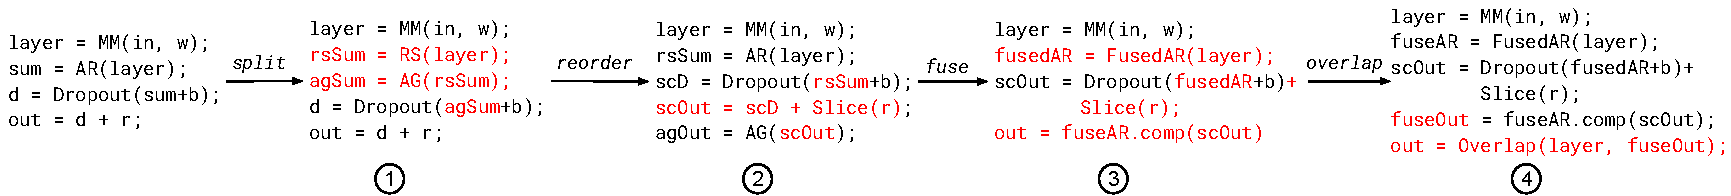
\includegraphics[width=\linewidth]{figures/coconet-example.pdf}
  \caption{\tool programs produced by performing transformations on the program of Figure~\ref{fig:traditional-mp}. Each schedule can be represented as a standalone program. Lines in \textcolor{red}{red} highlights changes at a step. (\texttt{AR}: AllReduce, \texttt{AG}: AllGather, and \texttt{RS}: ReduceScatter)
%  	to the program produced after applying the transformation.
  	\label{fig:mp-schedules}}
    \vspace{-1em}
\end{figure*}

\section{\tool Transformations}
\label{sec:schedule}
\tool provides four semantics preserving \emph{transformations} to optimize a program written in the DSL.
All transformations are valid based on rules described in the sections below. 
\tool automatically checks the validity of each transformation based on these rules and throws an error for  an invalid transformation.

We call an order of transformations a \emph{schedule}.
A user can manually specify the schedule to optimize the program.
Additionally, a user can invoke the autotuner to automatically find the best performing schedule for the given problem sizes and the underlying architecture.
Below we present each transformation by applying them on the program from Figure~\ref{fig:traditional-mp} and show equivalent \tool{} programs generated after applying each transformation in Figure~\ref{fig:mp-schedules}.

\subsection{Splitting Communication}
The \texttt{split} transformation breaks a collective communication operation into two communication operations.
One of the two split policies supported by \tool is

\textbf{AllReduce Split RS-AG} splits an \allreduce into a \reducescatter to produce a \sliced tensor and an \allgather on the \sliced tensor to return a \replicated tensor.

% \textbf{AllReduce Split B-R} splits an \allreduce into a \reduce to produce a tensor on user specified root rank and then \broadcast this tensor to all ranks in \WORLD.

\spara{Running Example} The \allreduce in Figure~\ref{fig:traditional-mp} is split into \texttt{rsSum} that does a \reducescatter on \texttt{layer} and \texttt{agSum} that does an \allgather on \texttt{rsSum}.
{
\small
\begin{lstlisting}[language=DSL,numbers=none]
(rsSum, agSum) = split(layer, ARSplitRSAG);
\end{lstlisting}
}

The program \circled{1} of Figure~\ref{fig:mp-schedules} is the implementation of this schedule where the input to Dropout is replaced by \texttt{agSum}.

\spara{\textit{Validity}} Since an \allreduce can always be split to a \reducescatter and an \allgather, this transformation is always valid.

\begin{figure}[t]
	\centering
	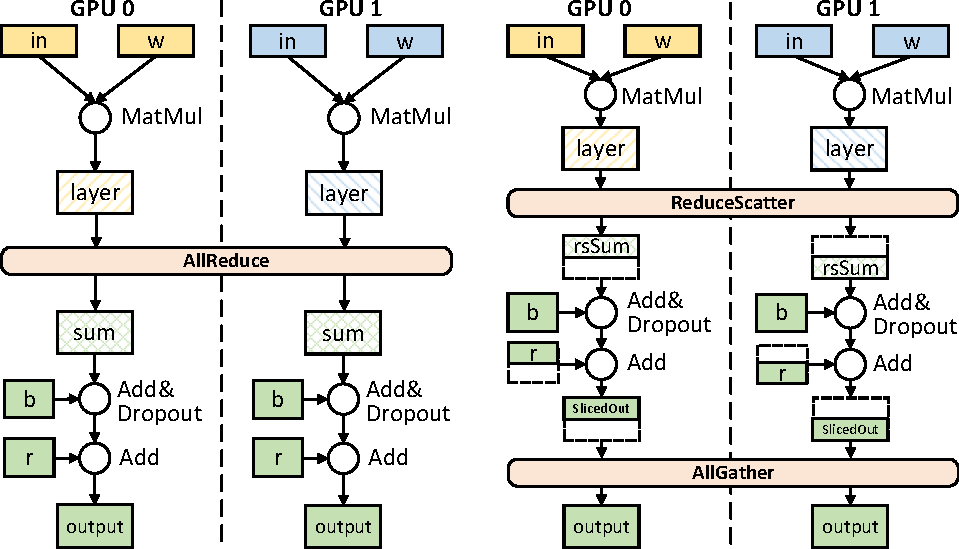
\includegraphics[width=.9\linewidth]{figures/reduceScatter}
%	\caption{Example of parallel Self-Attention layer on two GPUs using AllReduce (on left) and using ReduceScatter + AllGather (on right).}
	\caption{Equivalent programs (from Figure~\ref{fig:traditional-mp}) using AllReduce (on left) or using ReduceScatter + AllGather (on right).}
	\label{fig:model-parallel-using-reducescatter}
\end{figure}

\subsection{Reordering Operations}
The \texttt{reorder} transformation swaps operations with an \allgather or a \broadcast in the DFG of a program.
We explain this transformation for \allgather below: 

\textbf{AllGather Reorder} reorders an \allgather with communication and computation operations. 
This transformation changes the layout of the operations, the input and output of operations, and the input and output of the \allgather.
We explain this transformation below using the running example.

% \textbf{Broadcast Reorder} is similar to \allgather reorder except that it requires the user to specify a root rank.

\spara{Running Example}
In Figure~\ref{fig:mp-schedules}, applying the \texttt{reorder} transformation changes the program \circled{1} to \circled{2} by reordering \allgather (\texttt{agSum}) with computations \texttt{d} and \texttt{out}.
The reorder transformation replaces these operations in the DFG with three new operations: \texttt{scD} and \texttt{scOut},
both of which performs sliced computations, and \texttt{agOut}, which gathers the final result of computations.
{
  \small
\begin{lstlisting}[language=DSL,numbers=none]
(scD, scOut, agOut) = reorder(d, out, agSum);
\end{lstlisting}
}
The new sliced computations perform the same operations as original computations with two differences: (i) the output of \allgather used in the computation is replaced by the input of \allgather, and (ii) since the input of \allgather is sliced, 
all tensors input to the computations are also sliced along the same dimension as the input of \allgather.
After reorder, \texttt{scD} performs the same computation as \texttt{d} but \texttt{scD} takes \texttt{rsSum} and \texttt{Slice(r)} as input.
Therefore, the layout of \texttt{scOut} is also sliced while the computation is same as \texttt{out}.
Furthermore, the new \allgather is performed on the outputs of the computations, for example, 
after reorder, the \allgather (\texttt{agOut}) is performed on \texttt{scOut}.
Figure~\ref{fig:model-parallel-using-reducescatter} shows the workflow of this schedule.
% Here the input to Dropout is now the output of \reducescatter (\texttt{rsSum}) and computations are performed on slice of residual (\texttt{r}) to produce a sliced output.
% Then, \allgather collects the sliced output to obtain a replicated output.
% The next section describes fusion of communication and computation. 

\spara{\textit{Validity}} The \texttt{reorder} transformation is valid only if operations being reordered with an \allgather can be sliced along the dimension the \allgather is performed.
The rules of slicing an operation depend on the type of operation and the dimensions of inputs to the operations.
For example, \texttt{d} and \texttt{out} can be sliced because the computations have the same dimensions as \texttt{agOut}.
Section~\ref{sec:opt-workloads} shows how P2P Send can be reordered with an \allgather.
% A MatMul can be sliced in the rows or columns dimension of the output matrix but not in the reduction dimension.

\subsection{Fusing Operations}
\label{sec:sched:fusion}

Fusing multiple computations is a common technique used by existing compilers~\cite{tvm18,distributed-halide,fireiron,polymage-gpu,halide}.
\tool extends this concept to fuse multiple computations and communications in a single operation and provides this capability using the \texttt{fuse} transformation.
Below we explain two fuse policies supported by \tool:

\textbf{Computation Fuse} fuses a series of computations in a single operation that performs all these operations.

\textbf{AllReduce Fuse} fuses a series of \reducescatter, sliced computations, and \allgather operations in a single Fused\allreduce that performs all these operations.

\spara{Running Example}
We can fuse \reducescatter (\texttt{rsSum}), computations (\texttt{scD} and \texttt{scOut}), and \allgather (\texttt{agOut}) in program \circled{2} of Figure~\ref{fig:mp-schedules} into a Fused\allreduce to obtain program \circled{3}.
{
\small
\begin{lstlisting}[language=DSL,numbers=none]
fuseAR = fuse(rsSum, scOut, agOut, ARFuse);
\end{lstlisting}
}
The \texttt{comp} method of \texttt{fusedAR} specifies the computation to be fused with Fused\allreduce and returned \texttt{out} is the output.

\spara{\textit{Validity}} Fusing multiple operations into one operation is valid only if the dependencies in the DFG after fusion are preserved.

\subsection{Overlapping Operations}
\tool provides the \texttt{overlap} transformation to overlap a series of producer-consumer operations to utilize multiple resources of hardware simultaneously.
% One use case of this transformation is to overlap computation and communication operations.
% It takes two or more operations as input and returns a single operation.

\spara{Running Example} 
In the program \circled{3} of Figure~\ref{fig:mp-schedules} we overlap the matrix multiplication (\texttt{layer}) with Fused\allreduce (\texttt{fuseAR}) to obtain program in \circled{5}.
{
\small
\begin{lstlisting}[language=DSL,numbers=none]
layerWithAR = overlap(layer, fusedAR);
\end{lstlisting}
}

\spara{\textit{Validity}} Overlapping multiple operations is valid only when all operations have a producer-consumer relationship between them.

% Operation returned by \texttt{Overlap} is the final output of the program.

\subsection{Automatic Exploration of Schedules}
\tool provides an \emph{autotuner} to automatically explore the space of all schedules of a program and return the schedule that provides the best performance for the underlying architecture and input sizes.
First, the autotuner fuses all pointwise computations up to a pre-defined threshold to decrease the search space and then exhaustively explores the schedule space in a breadth first search manner.
Finally, the autotuner generates code for all schedules in its search space, executes all programs, and returns the schedule with minimum execution time.
Table~\ref{tab:loc-autotuner-time} shows that the autotuner takes only a few seconds to explore the schedule space for all workloads.

\begin{figure}
  \small
  \centering
% Scalar lr(FP32), beta1(FP32), beta2(FP32);|\label{line:adam:scalars}|
% Tensor g(FP32, WORLD_SZ, SIZE, Sliced); |\label{line:adam:inputensor-begin}||\label{line:adam:continuous-tensor}|
% Tensor p(FP32, WORLD_SZ, SIZE, Replicated);
% Tensor m(FP32, WORLD_SZ, SIZE, Replicated);
% Tensor v(FP32, WORLD_SZ, SIZE, Replicated);|\label{line:adam:inputensor-end}| 
  \begin{subfigure}[t]{\columnwidth}
\begin{lstlisting}[language=DSL, numbers=left]
Var avg = AllReduce("+", g); |\label{line:adam:avg}|
Var m_ = Update(m, (m*beta1+(1-beta1)*avg));|\label{line:adam:pointwise-begin}||\label{line:update:m}|
Var v_ = Update(v, (v*beta2+(1-beta1)*avg*avg));|\label{line:update:v}|
Var m1 = m_/(1-Pow(beta1, t));
Var v1 = v_/(1-Pow(beta2, t));
Var p_ = Update(p, (p - lr * m1/(Sqrt(v1))));|\label{line:adam:pointwise-end}|

Execute adam({g,p,v,m,lr}, {p_});
\end{lstlisting}
\caption{Traditional implementation where 
               tensors \texttt{g} is local to each rank and \texttt{p},\texttt{m}, and \texttt{v} are replicated on all ranks.}
\label{fig:traditional-adam}
\end{subfigure}
\par\bigskip % Do not remove this. Without this there is no space between caption of above figure and the next figure. WEIRD bug. Never saw this in subfigure.
\begin{subfigure}[b]{\columnwidth}
\begin{lstlisting}[language=DSL, numbers=left]
comps = fuse(m_, v_, m1, v1, p_, 
             ComputationFuse);|\label{line:adam-schedule:fuse-comp}|
(rsG, agG) = split(avg, ARSplitRSAG); |\label{line:adam-schedule:split}|
(scComp, agP, agM, agV) = reorder(agG, comps, 
                                  AGReorder);|\label{line:adam-schedule:reorder}|  
asSlice(m); asSlice(v); dead(agM); dead(agV); |\label{line:adam-schedule:slice-m-v}| |\label{line:adam-schedule:remove-m-v-allgather}|
fuseAR = fuse(rsG, scComp, agP, AllReduceFuse);|\label{line:adam-schedule:fuse-allreduce}|
\end{lstlisting}
\caption{An Optimized Schedule. Tensors \texttt{g} is local, \texttt{p} is replicated on all ranks, while 
\texttt{m} and \texttt{v} are sliced among all ranks.}
\label{fig:adam-schedule}
\end{subfigure}
% Scalar lr(FP32), beta1(FP32), beta2(FP32);|\label{line:adam:scalars}|
% Tensor g(FP32, WORLD_SZ, SIZE, Sliced); |\label{line:adam:inputensor-begin}||\label{line:adam:continuous-tensor}|
% Tensor p(FP32, SIZE, Replicated);
% Tensor m(FP32, SIZE, Sliced);
% Tensor v(FP32, SIZE, Sliced);|\label{line:adam:inputensor-end}| 
% \hfill{}
% \begin{subfigure}{0.32\textwidth}
%   \begin{lstlisting}[language=DSL, numbers=left]
% avg = FusedAllReduce("+", g); |\label{line:adam:avg}|
% scP_ = p.update(p - scDiff);
% p_ = fuseAR.comp(scP_);

% adam({g,p,v,m,lr}, {p_});
%   \end{lstlisting}
% \caption{Equivalent \tool implementation after applying the schedule. 
% Tensors \texttt{g} and \texttt{p} are replicated on all ranks, while 
% \texttt{m} and \texttt{v} are sliced among all ranks. \texttt{scDiff}
% represents the sliced \texttt{diff}. \label{fig:optimized-adam}}
% \end{subfigure}
  \caption{Optimizing parameter update using Adam in \tool. 
  The implementation takes four input tensors: parameters (\texttt{p}), gradients (\texttt{g}),
  momentum (\texttt{m}), and velocity (\texttt{v}).
  \label{fig:optimizing-adam}}
  \end{figure}

\section{Distributed Workloads in \tool}
\label{sec:opt-workloads}
We additionally optimized two distributed machine learning workloads using \tool: (i) parameter update using Adam~\cite{adam}, and (ii) point-to-point communication in pipeline parallelism.

\spara{Adam in Data Parallel Training}: Figure~\ref{fig:traditional-adam} shows the traditional implementation of parameter update using Adam.
First, all ranks average the gradients using \allreduce and then perform computations to update the optimizer state and model parameters.
\texttt{Update} updates the values of a tensor and reflects the new values in that position in the DFG (lines~\ref{line:update:m}--\ref{line:update:v}).
Figure~\ref{fig:adam-schedule} presents a schedule that optimizes this by distributing the computation on all ranks in a single kernel.
Line~\ref{line:adam-schedule:fuse-comp} fuses all computations in \texttt{comps}.
Line~\ref{line:adam-schedule:split} splits the \allreduce into a \reducescatter and an \allgather, such that computations take output of \allgather (\texttt{agG}) as input.
Line~\ref{line:adam-schedule:reorder} reorders \allgather with computations, such that,
each rank performs computations on a slice of tensors.
% \allgather operations are returned for parameters and optimizer state.
Line~\ref{line:adam-schedule:slice-m-v} slices optimizer states on all ranks to decrease memory usage and removes corresponding \allgather.
Finally, line~\ref{line:adam-schedule:fuse-allreduce} fuses all operations in a single kernel.

\begin{figure}[t]
  \begin{subfigure}{\columnwidth}
  \centering
  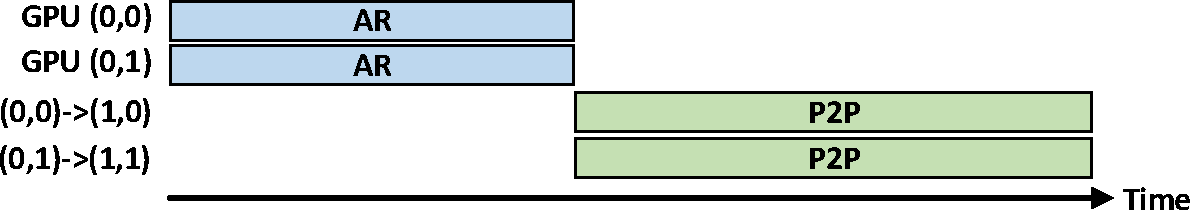
\includegraphics[width=.85\linewidth]{figures/pipeline-p2p-fusion-1.pdf}  
  \caption{In Megatron-LM each GPU sends redundant data. \label{fig:p2p-fusion-1}}
\end{subfigure}
\par\bigskip % Do not remove this. Without this there is no space between caption of above figure and the next figure. WEIRD bug. Never saw this in subfigure.
\begin{subfigure}{\columnwidth}
  \centering
  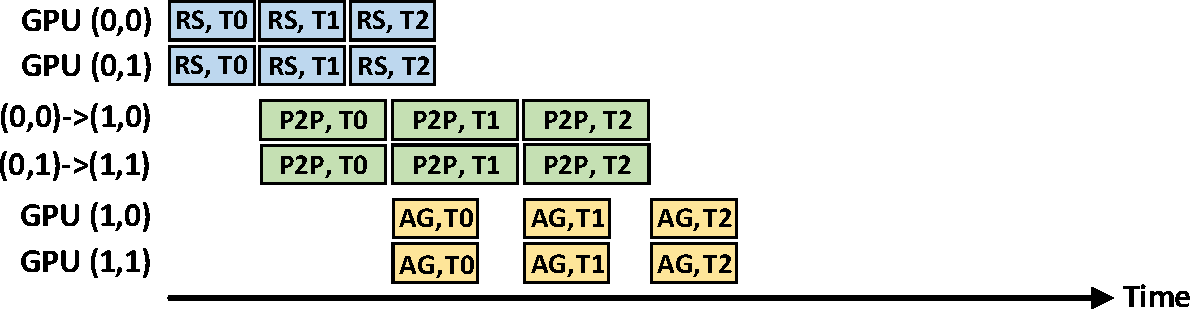
\includegraphics[width=.85\linewidth]{figures/pipeline-p2p-fusion-3.pdf} 
  \caption{Communication operations can be overlapped at the granularity of each 
  \emph{communication buffer tile} of data in single kernel 
  call.\label{fig:p2p-fusion-3}}
\end{subfigure}
  \caption{Two different schedules of pipeline parallelism.
\label{fig:P2Ptimeline}}
\end{figure}

\spara{Point-to-Point Communication in Pipeline Parallelism}: 
Figure~\ref{fig:p2p-fusion-1} shows a scenario of pipeline parallelism in Megatron-LM
with two transformer layers assigned to two groups each with two ranks. 
Rank $i$ in group $j$ is shown by $(j,i)$.
Each group uses model parallelism within its transformer layer.
Pipeline parallelism in Megatron-LM works as follows.
First, all ranks in the first group reduce their input using 
\allreduce to get replicated output.
Then each rank performs pointwise computations over the replicated output.
Finally, the first group sends the result of computations to the corresponding rank in the
second group using point-to-point (P2P) sends. (Line~\ref{line:p2p:comp2} in Figure~\ref{fig:traditional-p2p} shows these computations but are omitted in Figure~\ref{fig:P2Ptimeline} for simplicity). Since the output of \allreduce in 
Figure~\ref{fig:p2p-fusion-1} is replicated, redundant data is sent using P2P.
We can avoid this redundant communication by splitting
the \allreduce to \reducescatter and \allgather and reordering the P2Ps with the
\allgather. 
Hence, the inter-group communication is reduced by 
the group size.
We can further optimize by overlapping all communication operations. 
Figure~\ref{fig:p2p-fusion-3} shows that if the 
buffers are split into multiple tiles (\texttt{T0}--\texttt{T2} in the figure), 
intra-group and inter-group communications can be overlapped.
%  to further reduce the communication time.

% Figure~\ref{fig:optimizing-p2p} shows how to do these 
% optimizations with \tool. 
Figure~\ref{fig:traditional-p2p} is the original program, 
while Figure~\ref{fig:p2p-schedule} optimizes it by applying transformations.
Line~\ref{line:p2p:fuse-send} fuses the P2P 
send with computations.
Line~\ref{line:p2p:split} splits the \allreduce and reorders the returned \allgather with the fused P2P send at Line~\ref{line:p2p:reorder}.
Hence, P2P send and computations are performed 
on only a slice of data on the next group where the \allgather is also performed.
Finally, all three new operations get overlapped in Line~\ref{line:p2p:fuseAR}.
% This overlapping can only be achieved by generating custom communication and computation kernels.
%Figure~\ref{fig:traditional-p2p} shows the implementation of pipeline parallelism in Megatron-LM.
%Here one Transformer layer is assigned to a group of consecutive ranks, such that each group uses model parallelism for the Transformer layer.
%First all ranks in a group perform reduces their input (\texttt{in}) using \allreduce to obtain a replicated output.
%Each rank in the group sends the output to same rank of next group using point-to-point (P2P) communication, over which several pointwise computations are done.
%Figure~\ref{fig:p2p-schedule} optimizes the program by avoiding send of redundant replicated output. 
%Lines~\ref{line:p2p:fuse-comp}--\ref{line:p2p:fuse-send} fuses the P2P send with computations.
%At line~\ref{line:p2p:reorder} \allreduce is split and the returned \allgather is reordered with fused send, so that, both P2P send and computations are performed on only a slice of data on the next group and the \allgather is also performed on the next group.
%Finally, all three new operations can be overlapped because \reducescatter and \allgather are performed in different groups and P2P send uses interconnect between the groups.

\begin{figure}[!t]
	\small
	\begin{subfigure}{\columnwidth}
		\begin{lstlisting}[language=DSL, numbers=left]
Var sum = AllReduce("+", in);
Var send = Dropout(recv+b,0.1) + r;|\label{line:p2p:comp1}||\label{line:p2p:comp2}|
Var output = Send(send, 
                  GroupRank(GROUP+1, RANK));

Execute transformer({in}, {output});
		\end{lstlisting}
		\caption{Traditional implementation. Each rank of a group sends same data to next group.}
		\label{fig:traditional-p2p}
	\end{subfigure}
	\par\bigskip % Do not remove this. Without this there is no space between caption of above figure and the next figure. WEIRD bug. Never saw this in subfigure.
	\begin{subfigure}{\columnwidth}
		\begin{lstlisting}[language=DSL, numbers=left]
fuseSend = fuse(send, output, SendFuse);|\label{line:p2p:fuse-send}|
(rsSum, agSum) = split(sum, ARSplitRSAG); |\label{line:p2p:split}|
(scSend, agOut) = reorder(fuseSend, agSum, 
                          AGReorder); |\label{line:p2p:reorder}|
overlapOut = overlap(rsSum, scSend, agOut); |\label{line:p2p:fuseAR}|
		\end{lstlisting}
		\caption{An Optimized Schedule. Each rank sends only a slice of data to ranks in next group and all operations are overlapped.}
		\label{fig:p2p-schedule}
	\end{subfigure}
	\caption{Optimizing pipeline parallelism of Megatron-LM. Input tensors: layer output \texttt{in}, bias \texttt{b}, and residual \texttt{r}. \label{fig:optimizing-p2p}}
\end{figure}


\iffalse

\begin{figure*}[t]
    \small
\begin{subfigure}{0.49\textwidth}
    \begin{lstlisting}[language=DSL]
    Variable lr(Float);
    Variable m(Float);
    Tensor g(Float, SIZE, GPUs);
    Tensor p(Float, SIZE, GPUs);
    Tensor v(Float, SIZE, GPUs);
    
    Stage sum = AllReduce("+", g);
    Stage v_ = m * v + sum/GPUs;
    Stage p_ = p - lr * v_;
    
    Pipeline pipeline({g, p, m, lr}, {v}, {p_});
\end{lstlisting}
\caption{Optimizing  SGD in \tool }
    \label{fig:traditional-sgd}
\end{subfigure}

\begin{subfigure}{0.45\textwidth}
\begin{lstlisting}[language=DSL]     
        Stage sumRS;
        Stage sumAG;
        pipeline.split(sum, &sumRS, &sumAG, 
                       ReduceScatterAllGather); 
\end{lstlisting}
\caption{}
\end{subfigure}
\begin{subfigure}{0.45\textwidth}
        \begin{lstlisting}[language=DSL]     
                sumRS = ReduceScatter(g); 
                sumAG = AllGather(sumRS)
                //Replace all references of 
                //sum with sumAG
        \end{lstlisting}
        \caption{}
\end{subfigure}

\begin{subfigure}{0.45\textwidth}
\begin{lstlisting}[language=DSL]     
        Stage v1_, vAG;
        pipeline.reorder(v_, sumAG, v1_, vAG); 
\end{lstlisting}
\caption{}
\end{subfigure}
\begin{subfigure}{0.45\textwidth}
        \begin{lstlisting}[language=DSL]     
                v1_ = m * slice(v) + sumRS/GPUs; 
                vAG = AllGather(v1_);
                p_ = p - lr * vAG;
        \end{lstlisting}
        \caption{}
\end{subfigure}

\begin{subfigure}{0.45\textwidth}
\begin{lstlisting}[language=DSL]     
        Stage p1_, pAG;
        pipeline.reorder(vAG, p_, p1_, pAG); 
        pipeline.asSlice(v); 
        pipeline.fuse({sumRS, v1_, p1_, pAG}, 
                      AllReduce); 
        pipeline.storeAt({p_, p},{v_, v});
\end{lstlisting}
\caption{}
\end{subfigure}
\begin{subfigure}{0.45\textwidth}
\begin{lstlisting}[language=DSL]     
        v1_ = m * slice(v) + sumRS/GPUs; 
        pAG_ = slice(p) - lr * v1_; 
        p1_ = AllGather(pAG_);
\end{lstlisting}
\caption{}
\end{subfigure}

\begin{subfigure}{0.45\textwidth}
\begin{lstlisting}[language=DSL]     
        pipeline.asSlice(v); 
        pipeline.fuse({sumRS, v1_, p1_, pAG}, 
                        AllReduce); 
        pipeline.storeAt({p1_, p},{v1_, v});
\end{lstlisting}
\caption{}
\end{subfigure}
\caption{SGD with momentum}
\end{figure*}



\begin{figure*}[t]
    \small
\begin{subfigure}{0.49\textwidth}
    \begin{lstlisting}[language=DSL]
    Variable lr(Float);
    Variable m(Float);
    Tensor g(Float, SIZE, GPUs);
    Tensor p(Float, SIZE, GPUs);
    Tensor v(Float, SIZE, GPUs);
    Tensor m(Float, SIZE, GPUs);
    
    Stage sum = AllReduce("+", g);
    Stage m_ = beta1 * m + (1-beta1)*sum;
    Stage v_ = beta2 * v + (1-beta2)*(sum*sum);
    Stage p_ = p - lr * m_/(1-beta1)/(sqrt(v_/(1-beta2)));
    
    Pipeline pipeline({g, p, m, lr}, {v}, {p_});
\end{lstlisting}
\caption{Optimizing  Adam in \tool }
    \label{fig:traditional-sgd}
\end{subfigure}

\begin{subfigure}{0.45\textwidth}
\begin{lstlisting}[language=DSL]     
        Stage sumRS;
        Stage sumAG;
        pipeline.split(sum, &sumRS, &sumAG, 
                       ReduceScatterAllGather); 
\end{lstlisting}
\caption{}
\end{subfigure}
\begin{subfigure}{0.45\textwidth}
        \begin{lstlisting}[language=DSL]     
                sumRS = ReduceScatter(g); 
                sumAG = AllGather(sumRS)
                //Replace all references of 
                //sum with sumAG
        \end{lstlisting}
        \caption{}
\end{subfigure}

\begin{subfigure}{0.45\textwidth}
\begin{lstlisting}[language=DSL]    
        Stage mv;
        pipeline.fuse({m_,v_}, mv) ;
        Stage mv_, mvAG;
        pipeline.reorder(mv_, sumAG, mv1_, mvAG); 
\end{lstlisting}
\caption{}
\end{subfigure}
\begin{subfigure}{0.45\textwidth}
        \begin{lstlisting}[language=DSL]     
                Stage m_ = beta1 * slice(m) + (1-beta1)*sumRS;
                Stage v_ = beta2 * slice(v) + (1-beta2)*(sumRS*sumRS);
                vAG = AllGather(v1_);
                mAG = AllGather(m1_);
                p_ = p - lr * f(mAG, vAG);
        \end{lstlisting}
        \caption{}
\end{subfigure}

\begin{subfigure}{0.45\textwidth}
\begin{lstlisting}[language=DSL]     
        Stage p1_, pAG;
        pipeline.reorder(mvAG, p_, p1_, pAG); 
        pipeline.asSlice(v); 
        pipeline.asSlice(m); 
        
\end{lstlisting}
\caption{}
\end{subfigure}
\begin{subfigure}{0.45\textwidth}
\begin{lstlisting}[language=DSL]     
        v1_ = m * slice(v) + sumRS/GPUs; 
        pAG_ = slice(p) - lr * v1_; 
        p1_ = AllGather(pAG_);
\end{lstlisting}
\caption{}
\end{subfigure}

\begin{subfigure}{0.45\textwidth}
\begin{lstlisting}[language=DSL]     
        pipeline.asSlice(v); 
        pipeline.fuse({sumRS, v1_, p1_, pAG}, 
                        AllReduce); 
        pipeline.storeAt({p1_, p},{v1_, v});
\end{lstlisting}
\caption{}
\end{subfigure}
\caption{Adam}
\end{figure*}


\begin{figure*}[t]
        \small
\begin{subfigure}{0.49\textwidth}
        \begin{lstlisting}[language=DSL]
        Variable lr(Float);
        Variable m(Float);
        Tensor g(Float, SIZE, GPUs);
        Tensor p(Float, SIZE, GPUs);
        Tensor v(Float, SIZE, GPUs);
        Tensor m(Float, SIZE, GPUs);
        
        Stage sum = AllReduce("+", g);
        Stage m_ = beta1 * m + (1-beta1)*sum;
        Stage v_ = beta2 * v + (1-beta2)*(sum*sum);

        Stage r1 = Reduce("+", p * p);
        Stage p_upd = m_ / sqrt(v_ + eps) + lambda * p
        Stage r2 = Reduce("+", p_upd * p_upd)

        Stage p_ = p - r1/r2*lr* p_upd
        
        Pipeline pipeline({g, p, m, lr}, {v}, {p_});
    \end{lstlisting}
\end{subfigure}
\caption{LAMB}

\begin{subfigure}{0.49\textwidth}
        \begin{lstlisting}[language=DSL]
        Variable lr(Float);
        Variable m(Float);
        Tensor g(Float, SIZE, GPUs);
        Tensor p(Float, SIZE, GPUs);
        Tensor v(Float, SIZE, GPUs);
        Tensor m(Float, SIZE, GPUs);
        Stage p_slc = slice(p)


        Stage sumRS = ReduceScatter("+", g);
        Stage m_slc = beta1 * slice(m) + (1-beta1)*sumRS;
        Stage v_slc = beta2 * slice(v) + (1-beta2)*(sumRS*sumRS);
        Stage p_upd_slc = m_slc / sqrt(v_slc + eps) + lambda * p_slc

        Stage r1 = AllReduce("+", p_slc * p_slc);
        Stage r2 = AllReduce("+", p_upd_slc * p_upd_slc)

        Stage p_slc_ = p_slc - r1/r2*lr* p_upd_slc

        Stage p_ = AllGather(p_slc_)

        Pipeline pipeline({g, p, m, lr}, {v}, {p_});
    \end{lstlisting}
\end{subfigure}

\caption{Optimizing LAMB in \tool }
        \label{fig:lamb}
\end{figure*}

\tool automatically checks validity of each computation based on a set of \emph{validation rules}.
Each validation rule checks the properties of all tensors involved in the computation and assign values to all properties of the output tensor.
Figure~\ref{fig:rules} presents the validation rules for all computations supported by \tool.
In the validation rules the four properties of a tensor (T) are represented as follows: (i) $\type{}$ is the type of elements, 
(ii) $n$ is the number of elements, (iii) $\Locs{}$ is the set of ranks, and (iv) $\alloc{}$ is the allocation type.
Below we explain the validation rules of all computations.

\paragraph{Pointwise Computations} Pointwise computations are valid only if the input tensors have same value of properties and the output tensor will have properties with these values (rules \textsc{E-BinaryOp} and \textsc{E-UnaryOp}).

\paragraph{Communication Collectives} Each computation involving a NCCL Communication Collective computations has a validation rule associated, which follows the semantics of the computation defined in the NCCL documentation~\cite{}.
\allreduce on the input tensor is valid only if the input is a \complete tensor and present on all ranks in the \WORLD (\textsc{E-AllReduce}). After \allreduce, the output tensor has same properties as the input tensor.
Similar to \allreduce, \reducescatter requires same conditions on the input tensor but the output tensor will be equally \sliced among all ranks in \WORLD (rule \textsc{E-ReduceScatter}).
Since \allgather gathers all slices from all ranks and stores these slices in \complete tensors on all ranks, \allgather requires input tensor to be a \sliced tensor stored on all ranks in \WORLD and the output tensor is a \complete (rule \textsc{E-AllGather}).
Slicing a tensor is possible only if it is continuous and the output tensor is stored on all ranks where the input tensor was stored (rule \textsc{E-Scatter}).
So far we have presented the validation rules that can be checked during the compile time.
However, the rules for allocation type for Reduce and Broadcast must be dynamically checked because both requires a particular rank as input, which must be checked at the runtime if it belongs to \WORLD.
These dynamic checks are automatically generated by \tool code generator (discussed in Section~\ref{sec:code-gen}).
\reduce can be called on tensors that are present on all ranks in \WORLD with the target rank in the \WORLD and the output tensor is available on the target rank only (rule \textsc{E-Reduce}).
On the other hand, Broadcast is valid only for \complete tensors and when all nodes in \WORLD will receive the output tensor(rule \textsc{E-Broadcast}).

\paragraph{LoadTensorAtRank}

\paragraph{ReduceTensor} Reducing a single tensor is possible on both \sliced or \complete tensors. However, the tensor must be stored on all ranks in \WORLD (rule \textsc{E-ReduceTensor}).
The output tensor will contain only one element, which will have different value for different ranks.

\paragraph{Cast} According to the validation rule \textsc{E-Cast} the  output tensor has same properties as the input tensor, except the output's element type is the argument of Cast.

\paragraph{Example} We illustrate type checking on \tool code in Figure~\ref{fig:FusedSGD} and Figure~\ref{fig:reduce-scatter-sgd}.
In Figure~\ref{fig:FusedSGD}, \allreduce produces a \complete stage of same size, element type, and on nodes.
Then the computations on lines~\ref{}--\ref{} again produces tensors with same properties. 
In contrast, Figure~\ref{fig:reduce-scatter-sgd} uses a \reducescatter to generate a tensor of size \aj{To be continued}

\begin{figure}[t]
  \small
\begin{subfigure}{\columnwidth}
\(
\begin{array}{@{}l@{}r@{\,}c@{\,}l@{}}
        \textbf{Tensors} & \tensor{}^{[\type{},n,\Locs{}, \alloc{}]}\\
        \text{Element Type} & \type{} & \in & \ldots\\ %\{u8, i8, f16, \cdots,  u64, i64, f64\} \\
        \text{Tensor Size} & n & \in & Z^{+} \\
        \text{Set of all ranks} & WORLD & \subseteq & Z^{+} \\
        \text{Set of Storage Locations} & \Locs{} & \subseteq & WORLD\\
        \text{Allocation Type} & \alloc{} & \in & \{\text{\complete, Sliced}\}\\
        \text{Pointwise Computations} & \texttt{op} & \in &{+, -, *, /, pow}\\
\end{array}
\)
\end{subfigure}

\begin{subfigure}{\columnwidth}
\begin{mathpar}
\inferrule*[Left=E-BinaryOp]
        {\tensor{}_{1}^{[\type{}_1,n_1,\Locs{}_1, \alloc{}_1]} = \texttt{op}(\tensor{}_{2}^{[\type{},n,\Locs{},\alloc{}]}, \tensor{}_{3}^{[\type{},n,\Locs{},\alloc{}]})}
        {\type{}_1 = \type{} \\ n_1 = n \\ \Locs{}_1 = \Locs{} \\ \alloc{}_1 = \alloc{}}\\ %\forall_{\loc{} \in \Locs{}}\forall_{0 \leq i \leq n} \tensor{}_{1}[\loc{}, i] = \texttt{op}(\tensor{}_{2}[\loc{}, i], \tensor{}_{3}[\loc{}, i])
\inferrule*[Left=E-UnaryOp]
        {\tensor{}_{1}^{[\type{}_1,n_1,\Locs{}_1, \alloc{}_1]} = \texttt{op}(\tensor{}_{2}^{[\type{},n,\Locs{},\alloc{}]})}
        {\type{}_1 = \type{} \\ n_1 = n \\ \Locs{}_1 = \Locs{} \\ \alloc{}_1 = \alloc{}}\\ %\forall_{\loc{} \in \Locs{}}\forall_{0 \leq i \leq n} \tensor{}_{1}[\loc{}, i] = \texttt{op}(\tensor{}_{2}[\loc{}, i], \tensor{}_{3}[\loc{}, i])
\inferrule*[Left=E-Slice]
        { {
          \begin{array}{ll}
            \tensor{}_{1}^{[\type{}_1,n_1,\Locs{}_1,\alloc{}_1]} = \texttt{Slice}(\tensor{}^{[\type{},n,\Locs{},\alloc{}]})\\
            \alloc{} = \complete
          \end{array}
        } }
        {
          {
            \begin{array}{ll}
              \type{}_1 = \type{} & n_1 = \frac{n}{|\Locs{}|} \\ 
              \Locs{}_1 = \Locs{} & \alloc{}_1 = \sliced
            \end{array}
          }
        }\\
\inferrule*[Left=E-Cast]
        {\tensor{}_{1}^{[\type{}_1,n_1,\Locs{}_1,\alloc{}_1]} = \texttt{Cast}(\tensor{}^{[\type{},n,\Locs{},\alloc{}]}, \type{}_2)}
        {\type{}_1 = \type{}_2 \\ n_1 = n \\ \Locs{}_1 = \Locs{} \\ \alloc{}_1 = \alloc{}}\\
\inferrule*[Left=E-LoadTensorAtRank]
        {\tensor{}_{1}^{[\type{}_1,n_1,\Locs{}_1,\alloc{}]} = \texttt{LoadTensorAtRank}(\tensor{}^{[\type{},n,\Locs{}, \alloc{}]}, \loc{}) \\ \alloc{} = \complete\\ \loc{} \in \Locs{}}
        {
          {
          \begin{array}{ll}
            \type{}_1 = \type{} & n_1 = n \\ 
            \Locs{}_1 = \{\loc{}\} & \alloc{} = \complete
          \end{array}
          }
        }\\

\inferrule*[Left=E-Reduce]
        {\tensor{}_{1}^{[\type{}_1,n_1,\Locs{}_1,\alloc{}]} = \texttt{Reduce}(\tensor{}^{[\type{},n,\Locs{}]}, \texttt{op}, \loc{}, \alloc{}) \\ \alloc{} = \complete\\ \Locs{} = \WORLDMath\\ \loc{} \in \Locs{}}
        {
          {
          \begin{array}{ll}
            \type{}_1 = \type{} & n_1 = n \\ 
            \Locs{}_1 = \{\loc{}\} & \alloc{} = \complete
          \end{array}
          }
        }\\
\inferrule*[Left=E-AllReduce]
        {\tensor{}_{1}^{[\type{}_1,n_1,\Locs{}_1,\alloc{}_1]} = \texttt{AllReduce}(\tensor{}^{[\type{},n,\Locs{},\alloc{}]}, \texttt{op}) \\ \alloc{} = \complete \\ \Locs{} = \WORLDMath}
        {
          {
          \begin{array}{ll}
            \type{}_1 = \type{} & n_1 = n \\ 
            \Locs{}_1 = \Locs{} & \alloc{}_1 = \complete %\forall_{0 \leq i \leq n} \forall_{\loc{} \in \Locs{}}\tensor{}_{1}[\loc{}, i] = \texttt{op}(\forall_{\loc_1{} \in \Locs{}} \tensor{}[\loc_1{}, i])
          \end{array}
          }
        }\\
\inferrule*[Left=E-ReduceScatter]
        {\tensor{}_{1}^{[\type{}_1,n_1,\Locs{}_1,\alloc{}_1]} = \texttt{ReduceScatter}(\tensor{}^{[\type{},n,\Locs{},\alloc{}]}, \texttt{op}) \\ \alloc{} = \complete\\ \Locs{} = \WORLDMath}
        {
          {
          \begin{array}{ll}
            \type{}_1 = \type{} & n_1 = \frac{n}{|\Locs{}|} \\
            \Locs{}_1 = \Locs{} & \alloc{}_1 = \sliced
          \end{array}
          }
        }\\%\forall_{0 \leq i \leq n_1} \forall_{\loc{} \in \Locs{}}\tensor{}_{1}[\loc{}, i] = \texttt{op}(\forall_{\loc_1{} \in \Locs{}} \tensor{}_{2}[\loc_1{}, i\times\loc_1{}])
\inferrule*[Left=E-AllGather]
        {
          {
            \begin{array}{ll}
            \tensor{}_{1}^{[\type{}_1,n_1,\Locs{}_1,\alloc{}_1]} = \texttt{AllGather}(\tensor{}^{[\type{},n,\Locs{},\alloc{}]})\\
            \Locs{} = \WORLDMath & \alloc{} = \sliced
            \end{array} 
          }
        }
        {
          {
            \begin{array}{ll}
              \type{}_1 = \type{} & n_1 = n\times|\Locs{}| \\
              \Locs{}_1 = \Locs{} & \alloc{}_1 = \complete
            \end{array}
          }
        }\\
\inferrule*[Left=E-Broadcast]
        {
          {
            \begin{array}{ll}
              \tensor{}_{1}^{[\type{}_1,n_1,\Locs{}_1,\alloc{}_1]} = \texttt{Broadcast}(\tensor{}^{[\type{},n,\Locs{}, \alloc{}]}, \loc{}_1) \\
              \loc{}_1 \in \WORLDMath
            \end{array}
          }
        }
        {
          {
            \begin{array}{ll}
              \type{}_1 = \type{} & n_1 = n \\
              \Locs{}_1 = \WORLDMath & \alloc{}_1 = \alloc{}\\
            \end{array}
          }
        }\\
\inferrule*[Left=E-ReduceTensor]
        {
          %{\begin{aligned}$\tensor{}_{1}^{[\type{}_1,n_1,\Locs{}_1,\alloc{}_1]} = \texttt{ReduceTensor}(\tensor{}^{[\type{},n,\Locs{}]}, \texttt{op},\alloc{}) \\ \Locs{} = \WORLDMath$\end{aligned}}
          {  
          \begin{array}{ll}
            \tensor{}_{1}^{[\type{}_1,n_1,\Locs{}_1,\alloc{}_1]} = \texttt{ReduceTensor}(\tensor{}^{[\type{},n,\Locs{}]}, \texttt{op},\alloc{}) \\
            \Locs{} = \WORLDMath
          \end{array}
          }
        }
        {
          {
            \begin{array}{ll}
            \type{}_1 = \type{} & n_1 = 1 \\ 
            \Locs{}_1 = \Locs{} & \alloc{}_1 = \alloc{}
            \end{array}
          }
        }
\end{mathpar}
\end{subfigure}
\caption{Validation rules for computations in \tool \label{fig:rules}}
\end{figure}

% Addressed: \mm{In Figure~\ref{fig:rules}, E-Scatter should take a  Continuous Tensor present in one node ($L = {l}$)?. Same issue for E-Broadcast.}
\iffalse
\section{Schedules in \tool}
\label{sec:schedule}
In \tool{} a user can create a schedule of a program by applying several transformations to the algorithm. 
Like in Halide~\cite{halide}, each transformation changes the code generated for the program but does not require any change to the original algorithm.
These transformations are based on rewrite rules for communication collectives and computations.
% In Section~\ref{sec:experiments}, we show that no one transformation performs best in all scenarios and different transformations provides best performance based on the tensor sizes and the size of \WORLD.

%In this section, we first describe the rewrite rules and then describe the transformations provided by \tool based on these rewrite rules.
\iffalse
\begin{table*}[t]
  \footnotesize
  % \begin{subtable}{\textwidth}
    \begin{tabular}[]{|l|l|l|l|}
      \hline
      Name & Input Stages  & Output Stages \\ \hline
      {\textsc{AllReduce} \textsc{Split 1}}  &$i_1 = AllReduce(t)$
        &$\begin{array}{l}o_1 = \reducescatter(t)\\ 
          o_2 = \allgather(o_1)\end{array}$\\ \hline
          {\textsc{AllReduce} \textsc{Fuse 1}} & 
          $\begin{array}{l}i_1 = \reducescatter(t)\\
            i_2 = \allgather(i_1)\end{array}$ & $o_1 = AllReduce(t)$\\\hline
            {\textsc{AllReduce} \textsc{Split 2}} &$i_1 = AllReduce(t)$ &  
        $\begin{array}{l}o_1 = Reduce(t, r)\\ 
        o_2 = Broadcast(o_1, r)\end{array}$\\\hline
      {\textsc{AllReduce} \textsc{Fuse 2}} & 
        $\begin{array}{l}i_1 = Reduce(t, r)\\ 
          i_2 = Broadcast(o_1, r)\end{array}$ & $o_1 = AllReduce(t)$\\\hline
          \thead{\textsc{AllGather}\textsc{Reorder}} &$\begin{array} {lcl}i_1 = \allgather(t)  
    \\i_2 = f(i_1, s) \end{array}$ &  $\begin{array} {lcl} o_1 = f(t, Slice(s)) 
    \\o_2 = \allgather(o_1)\end{array}$\\ \hline
    {\textsc{Broadcast} \textsc{Reorder}} & $\begin{array} {lcl} i_1 = Broadcast(t, r)  
      \\ i_2 = f(i_1, s)\end{array}$  & $\begin{array} {lcl} o_1 = f(i_1, Load(s, r))  
      \\ o_2 = Broadcast(o_1)\end{array}$\\\hline
       {\textsc{Fuse} \textsc{Computations}} & $\begin{array}{lcl} i_1 = f_1(t_1)  
    \\ i_2 = f_2(t_2) \\
    \ldots\\
    i_N = f_N(t_N)\end{array}$ & $\begin{array}{lcl} o_1 = FusedCompute(f_1, f_2, \ldots, f_N, \\
    ~~~~~~~~~~~~~~~~~~t_1, t_2,\ldots,t_N)\end{array}$\\ \hline
    \textsc{Fused\allreduce} & $\begin{array}{l}i_1 = \reducescatter(t)\\ 
    i_2 = f_1(i_1, s_1, s_2, \ldots)\\
    i_3 = \allgather(i_1)\end{array}$ & $\begin{array}{l} o_1 = FusedAllReduce(t, f_1, s_1, s_2, \ldots)\end{array}$\\ \hline
    \end{tabular}
  \caption{Each transformation in \tool takes some stages as inputs and produces new stages as outputs. \label{tab:rewrite-rules-transformations}}
\end{table*}

\begin{table*}
  \small
  % \begin{subtable}{\textwidth}
    \begin{tabular}[]{|l|l|l|l|l|}
      \hline
      \multicolumn{1}{|c|}{Rewrite Rule} & \multicolumn{3}{c|}{Transformation}\\ \hline
      &\multicolumn{1}{c|}{Name} & \multicolumn{1}{c|}{Input Stages}  & \multicolumn{1}{c|}{Output Stages} \\ \cline{2-4}
    \multirow{2}{*}{$AllReduce(t)\equiv AllGather(ReduceScatter(t))$}
        &\textsc{AllReduce Split 1}  &$i_1 = AllReduce(t)$
        &$\begin{array}{l}o_1 = \reducescatter(t)\\ 
          o_2 = \allgather(o_1)\end{array}$\\ \cline{2-4}
        & \textsc{AllReduce Fuse 1} & 
          $\begin{array}{l}i_1 = \reducescatter(t)\\
            i_2 = \allgather(i_1)\end{array}$ & $o_1 = AllReduce(t)$\\\hline
          \multirow{2}{*}{$\forall r \in \WORLDMath.~ AllReduce(t) \equiv Broadcast(Reduce(t, r), r)$}
        &\textsc{AllReduce Split 2} &$i_1 = AllReduce(t)$ &  
        $\begin{array}{l}o_1 = Reduce(t, r)\\ 
        o_2 = Broadcast(o_1, r)\end{array}$\\\cline{2-4}
        & \textsc{AllReduce Fuse 2} & 
        $\begin{array}{l}i_1 = Reduce(t, r)\\ 
          i_2 = Broadcast(o_1, r)\end{array}$ & $o_1 = AllReduce(t)$\\\hline
    $map(f, AllGather(t)) \equiv AllGather(map(f, t))$ & \textsc{AllGather Reorder} &$\begin{array} {lcl}i_1 = \allgather(t)  
    \\i_2 = f(i_1, s) \end{array}$ &  $\begin{array} {lcl} o_1 = f(t, Slice(s)) 
    \\o_2 = \allgather(o_1) \\ 
    o_3 = \allgather(t) \end{array}$\\ \hline
    $map(f, Broadcast(t))\equiv Broadcast(map(f, t))$ & \textsc{Broadcast Reorder} & $\begin{array} {lcl} i_1 = Broadcast(t, r)  
      \\ i_2 = f(i_1, s)\end{array}$  & $\begin{array} {lcl} o_1 = f(i_1, Load(s, r))  
      \\ o_2 = Broadcast(o_1) \\ 
       o_3 = Broadcast(t, r)\end{array}$\\\hline
    \end{tabular}
  % \end{subtable}

  % % \begin{subtable}{\textwidth}
  % %   \begin{tabular}[]{c|l|l|l|l|}
  % %     \hline
  % %     Rewrite Rule & \multicolumn{3}{c}{Transformation}\\ \hline
  % %     &Name & Input Stages  & Output Stages \\ \hline
  % %     $\begin{array}{lcllll} &AR(t) &\equiv& AG(RS(t)) && \text{AllReduce S/F 1} \end{array}$ &  \textsc{AllReduce Fuse 1} & $\begin{array} {lcl}i_1 = \reducescatter(t)  
  % %       \\i_2 = \allgather(i_1)\end{array}$ & $o_1 = AllReduce(t)$\\ \hline
  % %       $\begin{array}{lcllll}&AR(t) &\equiv& BC(Rd(t, r), r) \wedge r \in \WORLD& \text{AllReduce S/F 1} \end{array}$ &  \textsc{AllReduce Fuse 2} & $\begin{array} {lcl} i_1 = Reduce(t, r)  
  % %         \\ i_2 = Broadcast(o_1, r)\end{array}$ & $o_1 = AllReduce(t)$\\
  % %     \hline
  % %   \end{tabular}
  % %   \caption{Fuse Transformations\label{tab:fuse-trans} \aj{Show fused pointwise computations?}}
  % % \end{subtable}

  % \begin{subtable}{\textwidth}
  %   \begin{tabular}[]{|l|l|l|l|l|}
  %     \hline
  %     Rewrite Rule & \multicolumn{3}{c}{Transformation}\\ \hline
  %     &Name & Input Stages  & Output Stages \\ \hline
  %     $\begin{array}{lcllll} &map(f, AG(t)) &\equiv& AG(map(f, t)) && \textsc{C-AllGather} \end{array}$ & \textsc{AG} &$\begin{array} {lcl}i_1 = \allgather(t)  
  %       \\i_2 = f(i_1, s) \end{array}$ &  $\begin{array} {lcl} o_1 = f(t, Slice(s)) 
  %       \\o_2 = \allgather(o_1) \\ 
  %       o_3 = \allgather(t) \end{array}$\\ \hline
  %       $\begin{array}{lcllll} &map(f, BC(t)) &\equiv& BC(map(f, t)) && \textsc{C-Broadcast} \end{array}$ & \textsc{BC} & $\begin{array} {lcl} i_1 = Broadcast(t, r)  
  %         \\ i_2 = f(i_1, s)\end{array}$  & $\begin{array} {lcl} o_1 = f(i_1, Load(s, r))  
  %         \\ o_2 = Broadcast(o_1) \\ 
  %          o_3 = Broadcast(t, r)\end{array}$\\
  %     \hline
  %   \end{tabular}
  %   \caption{Reorder Transformations \label{tab:fuse-trans}}
  % \end{subtable}

  \caption{Rewrite rules and their corresponding transformations in \tool. Each transformation takes some stages as inputs and produces new stages as outputs. \label{tab:rewrite-rules-transformations}}
\end{table*}
\fi

\subsection{Identities}
The rewrite rules in \tool follow from a core set of identities on the primitives. First, these primitives are inverse of each other:
\begin{center}
  $
\begin{array}{ll}
  slice(join(sl)) &\iff sl\\
  join(slice(l)) &\iff l\\
  repl(drop(sl)) &\iff sl\\
  drop(repl(l))  &\iff l\\
  load(store(l,r)) & \iff l\\
  store(load(ll), rank(ll)) & \iff ll
\end{array}
$
\end{center}
Another important set of primitives rely on the commutativity of computation with tensor layout changes. Specifically:
\begin{center}
  $
\begin{array}{ll}
  map(f, repl(l)) &\iff repl(map(f, l))\\
  map(f, drop(rl)) &\iff drop(map(f, rl))\\
  map(f, join(sl)) &\iff join(map(f, sl))\\
  map(f, slice(l)) &\iff slice(map(f, l))\\
  map(f, load(ll)) &\iff load(map(f, ll))\\
  map(f, store(l, r)) &\iff store(map(f, l), r)
\end{array}
$
\end{center}
Finally, we use function composition as a way to fuse functions.
$$ map(f, map(g, l)) \iff map(f \circ g, l)$$

\subsection{Rewrite Rules}
We use the identities to 
%Rewrite rules allows rewriting of a \emph{source} computation sequence into a \emph{target} computation sequence ensuring that the output of target sequence is same as source sequence.
%We now 
explain four useful rewrite rules.

\subsubsection{Split/Fuse Communication Rewrite rules} 
A source sequence of one communication collective can be \emph{split} into a target sequence containing two or more communication collectives. 
Conversely, a source sequence with more than one communication collectives can be \emph{fused} into a target sequence containing a single communication collectives.
We focus on split/fuse rules for \allreduce, which can be split and fused in two different ways.

First, \allreduce on a tensor can be rewritten into a target sequence that first performs a \reducescatter on the tensor to produce \sliced tensors and then performs an \allgather computation on these \sliced tensors to obtain a \replicated tensor.
Conversely, a source sequence of \reducescatter and \allgather can be rewritten into a single \allreduce.
Our functional primitives expresses these rewrite rules.
%By applying \allgather on the output of \reducescatter in functional primitives, we obtain \allreduce.
Similarly, by applying $slice$ on the output of $reduce$ and then replication using $repl$ and $join$, we get \reducescatter and \allgather.
Hence, in terms of functional primitives this split/fuse rewrite rule is represented as:
$$repl(join(slice(reduce(l, f))) \iff repl(reduce(l, f))$$

Second, we can split \allreduce on a tensor into a sequence of \reduce and \broadcast, which first reduces the tensor on one of the ranks in \WORLD and then broadcasts this tensor to all ranks in \WORLD.
Conversely, a source sequence of \reduce and Broadcast can be rewritten to into a single \allreduce.
Using functional primitives this rewrite rule is represented as:
\[
  repl(load(store(reduce(l, f), r))) \iff repl(reduce(l, f))
\]


% These rules are semantics preserving. First two rules in Figure~\ref{fig:split-fuse-rules} represents the split of \allreduce into two other communication collective computations and fusion of these collective computations into \allreduce.
% According to \emph{AllReduce S/F 1}, \allreduce on a tensor $t$ is equivalent to \reducescatter on $t$ to produce a sliced tensor and then \allgather on that sliced tensor.
% This rewrite rule is semantics preserving because of two reasons.
% First, this rewrite rule follows the validation rules of \allreduce, \reducescatter, and \allgather.
% Second, the reduction done by \allreduce for an element is equal to the reduction done by \reducescatter for that element according to NCCL semantics.
% Similarly, second rule, says that \allreduce on a tensor $t$ is equivalent to Reduce on $t$ to some rank $r$ and Broadcast of the result from rank $r$ to all ranks in \WORLD.
% Similarl to previous rewrite rule, this rule is also semantics preserving because it follows the validation rules of \allreduce, Broadcast and Reduce if the rank $r$ is inside \WORLD, and reduction of each element by \allreduce is equal to the reduction by Reduce according to NCCL semantics.
% Hence, we can rewrite a combination of Broadcast and Reduce into \allreduce and vice-versa.

% \aj{These two are most important. There are others too. Like $Reduce(t,r) \iff AllReduce(t,r).load(r)$ Not sure should we mention them or not.}

\subsubsection{Commutativity Rewrite rules} 
A source sequence can be \emph{reordered} to create a target sequence, which specify new execution order of computations of the source.
We define two commutativity rewrite rules.
The first rule takes a source sequence where a computation is performed on the output of \allgather.
This source sequence can be converted to a target sequence, where the computation is performed on the input of \allgather and the \allgather is performed on the output of the computation.
Since input of \allgather is a \sliced tensor, the computation is also performed on the \sliced tensor.
Furthermore, the converse of the above reorder is also possible.
In the form of our functional primitives, this rule can be written as:
\[
  map(f, repl(join(l))) \iff repl(join(map(f, l)))
\]
The second rule reorders a source sequence where a computation is performed on the output of \broadcast into a target sequence where computation is performed on the input of \broadcast and \broadcast is performed on the output of the computation.
In the form of functional primitives, this rule can be written as:
\[
  map(f, repl(load(l)) \iff repl(load(map(f, l)))
\]
Commutativity rules are defined only for \allgather and \broadcast because these two 
collectives changes the layout of a tensor but other collectives also perform computations.

\subsubsection{Fuse Computations Rewrite Rules}
In general, many computations can be fused into a single one.
Existing DSLs~\cite{halide,lift-cgo17,lift-cgo18,distributed-halide}, fuse two computations into a single one to exploit memory locality.
We can represent such fusion using function composition ($\circ$)
\[
  map(f, map(g, l)) \iff map(f \circ g, l)
\]

\subsubsection{Fuse Computation-Communication Rewrite Rule}
\tool contains fused communication collectives, that fuses the computation acting on the output with the communication that produces it.
These collectives decrease the redundant reads and writes that come when a communication collective writes its output to global memory buffer and then the computation reads from that buffer.
Instead, in fused collectives the output element are passed through registers, removing expensive memory traffic.
Table~\ref{tab:fused-comm-collectives} presents the fused communication collectives supported in \tool and their representation as functional primitives.
For each collective, the computation $g$ is fused at a place, which is the first time in the collective when the output is produced.
For example, in Fused\reduce $g$ is performed over the output of $reduce$ by one rank because the output is produced for first time after $reduce$.
Similarly, in Fused\allreduce $g$ is performed on the output of $reduce$ and not on the output of $repl$.

We can rewrite sequences of computation and communication collectives into a single fused communication collective. 
One such rewrite rule fuses the computation on \reducescatter and the 
\allgather on the output of computation in Fused\allreduce.
We can represent this rewrite rule in the functional primitives as:
\begin{align*}
  repl(join(slice(map(g, reduce(l, f))))) \iff \\ repl(map(g, reduce(l, f)))
\end{align*}
\tool contains all such transformations based on these rewrite rules.

\begin{table}
  \small
  % \begin{subtable}{\textwidth}
    \begin{tabular}[]{|l|l|l|l|l|}\hline
      \thead{Fused Communication\\ Collective} & Functional Primitives \\ \hline
      Fused\reduce & $store(map(g, reduce(l, f), r))$ \\ \hline
      Fused\broadcast &  $repl(map(g, l))$ \\ \hline
      Fused\allreduce &  $repl(map(g, reduce(l, f)))$ \\ \hline
      Fused\reducescatter & $slice(map(g, reduce(l, f)))$ \\ \hline
      Fused\allgather& $repl(join(map(g, l)))$ \\ \hline
    \end{tabular}

  \caption{\tool's Fused Communication Collectives expressed using functional primitives. Each fused collective can have one or more computations fused in it. \label{tab:fused-comm-collectives}}
\end{table}
\fi

\iffalse 
\paragraph{Semantics Non-Preserving} Like transferring delta in 16-bits. \mm{We should make 16-bits the default. So all transformations are semantics preserving modulo precision requirements. Then we can elevate certain variables to fp32 to improve precision. }

Based on these rewrite rules, \tool provides two transformations that can be applied to one or more stages.
\fi
\fi
\section{The \tool Code Generator}
\label{sec:runtime}
\tool generates CUDA kernels for computation and communication operations for running on a distributed system with NVIDIA GPUs.
For each operation, \tool either generates (i) a call to a collective communication operation, 
(ii) a CUDA kernel for fused computations,
(iii) a CUDA kernel for fused-collective communications (Section~\ref{sec:code-gen-fused}), or
(iv) CUDA kernels for overlapping of communication and computation operations (Section~\ref{sec:overlap-impl}).
Moreover, \tool generates code for performing operations on multiple non-contiguous 
tensors (Section~\ref{sec:scattered-tensors}).
After generating CUDA kernels, \tool traverses the program's DFG to generate kernel calls.
\tool wraps generated programs as custom operators and integrates them into PyTorch, so that, applications like Megatron-LM can invoke them directly (Section~\ref{sec:pytorch-integration}).
We now discuss how \tool adapts NVIDIA Collective Communication Library (NCCL), a widely-used
hand-optimized high performance communication library, into a runtime
to execute above CUDA kernels. 
% NCCL is designed for single buffer tensor communications and is not built to execute arbitrary computations.

\subsection{NCCL Architecture}
\label{sec:nccl-arch}
NCCL communicates data stored in the global memory of one GPU to a memory location on another GPU using CUDA kernels.
NCCL's CUDA kernels perform communication by directly copying data from memory of one GPU to another GPU using GPUDirect Remote Data Memory Access~\cite{gpudirect}.
NCCL's architecture defines four key properties: (i) topology, (ii)
protocols, (iii) channels, and (iv) threads in a thread block of the
CUDA kernel. NCCL automatically sets key configuration values for these properties
based on the size of the input buffer, network architecture, and the size of
\WORLD. To ensure good performance, \tool's code generation must carefully reconfigure these properties
when extending NCCL to custom communication and computation.
We now provide a high level overview of these properties.

\spara{Topology} NCCL creates logical topologies, such as ring and tree, over the underlying interconnect network. 

\spara{Channels}
NCCL maps copies of a logical topology on the underlying interconnect network.
Each copy is called a channel and is assigned to one CUDA thread block.
% Each channel communicates by write to a fixed-size communication buffer stored on other GPU.

\spara{Protocols}
NCCL sends data using one of the three protocols: \texttt{LL}, \texttt{LL128}, and \texttt{Simple}.
These protocols make different tradeoffs between latency and bandwidth based on the type of inter-node synchronization used: 
\texttt{LL} has the lowest latency and \texttt{Simple} provides the highest bandwidth.
% NCCL chooses a protocol for each call based on the buffer size.

% Each protocol packs one or more elements of input into $N$-bits, where $N$ is equal or larger than the size of tensor type.
% This mechanism utilizes vector loads and stores for faster memory accesses and instruction level parallelism by 
% performing operations on multiple elements in consecutive instructions.
% LL and LL128 protocols have low latency but low bandwidth exchange speed where 
% LL packing data in 64-bits and LL128 packs data in 128-bits.
% Simple protocol packs data in 128-bits and is high bandwidth but incurs high latency, hence it is used for large sizes. 
% % It is able to achieve high GPU utilization.

\spara{Number of Threads}
NCCL sets a fixed number of threads for each channel (and thread block).
% The maximum depends on shared memory and register usage.
NCCL's kernels have high register usage, which limits the number of thread blocks per SM to one.

\spara{NCCL Workflow} 
After determining the topology, protocol, number of channels, and 
number of threads, NCCL calls its CUDA kernel for communication.
%Figure~\ref{fig:workflow-overlap} shows the operation of a \tool modified \allreduce NCCL kernel.
Each collective communication has three levels of tiling to fully utilize the massive parallelism of GPUs.
Data is first divided into \emph{buffer tiles} equal to the size of the communication buffer.
Each buffer tile is further divided among all ranks and channels to obtain \emph{chunks}.
Each channel communicates a chunk of data at a time.
The \emph{threads} in channels copy elements in and out of the buffers and
apply reduction operations (\texttt{sum}, \texttt{min}, \texttt{max}) if needed.
We now present details about \tool's code generation.

\subsection{Fused Collective Communications}
\label{sec:code-gen-fused}
Fused Collective Communication extends NCCL's existing kernels to enable arbitrary pointwise computations and reductions (i.e., beyond \texttt{min}, \texttt{max}, and \texttt{sum}).
We inspected more than 10K lines of code in NCCL to identify where computations can be added to pass intermediate values from communication to fused computations directly through registers.
\tool supports fusion of both pointwise operations and reductions into NCCL collectives.
% In future, we will extend the support of \tool to other stencil computations.

Each NCCL protocol utilizes a different mechanism for communication and
\tool generates code for all of them. The important features of a protocol are
the pack type (64-bit for \texttt{LL}, 128-bit for \texttt{LL128} and \texttt{Simple}) and 
the load/store access pattern (shared memory for LL128, global memory for \texttt{LL} and \texttt{Simple}).
% Moreover, \tool generated code for LL128 performs load and stores from shared memory, 
% which is the mechanism LL128 uses to improve its performance.
\tool generates template code for all element types in NCCL, and dispatches accordingly at runtime.
%which are selected by NCCL at the runtime according to the element type of tensor.
There are some subtleties in the code generation worth discussing:

\spara{Mixed Precision} 
When the element types of computations and the input tensors are different, \tool finds the largest element type and based on 
the pack type of the protocol calculates how many elements can be loaded at once.
All code will then be generated to operate on these many elements.

\spara{Sliced Tensor}
When a sliced tensor is used by a fused collective communication,
all memory accesses performed need to be mapped to elements of the sliced tensor.
\tool generates code that produces this mapping. 
To perform an \allgather on sliced tensors, the inverse of this mapping is
produced.

\spara{Tensor Reduction}
To reduce a \sliced tensor, each rank reduces locally and do an \allreduce.
This \allreduce reuses already established connections among ranks in the surrounding communication kernel to avoid extra startup latency.

\begin{figure*}[t]
	%https://docs.google.com/drawings/d/1yruTA_zsBAtsioXto2p7XsyDypk3WE8Dqx6Z4e9-35g/edit
	\centering
    \begin{subfigure}{0.48\linewidth}
    	\centering
    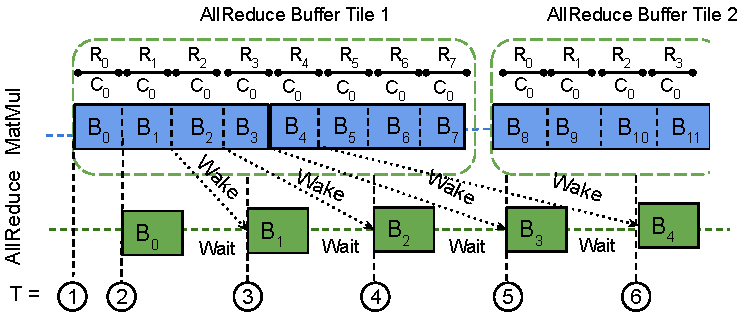
\includegraphics[width=\linewidth]{figures/overlap-example-rank-0.pdf}
    \caption{Workflow of overlap on \textbf{rank 0}. Rank 0 starts with chunk 0. }
	\end{subfigure}
    \hfill % \par \bigskip% Do not remove this. Without this there is no space between caption of above figure and the next figure. WEIRD bug. Never saw this in subfigure.
    \begin{subfigure}{0.48\linewidth}
    	\centering
        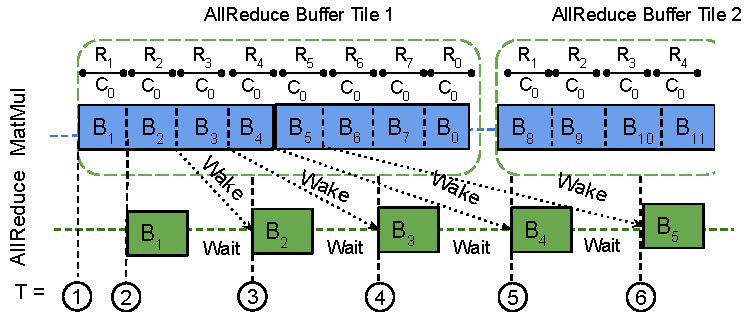
\includegraphics[width=\linewidth]{figures/overlap-example-rank-1.pdf}
        \caption{Workflow of overlap on \textbf{rank 1}. Rank 1 starts with chunk 1. }
    \end{subfigure}

	\caption{Workflow of \tool's overlapping of MatMul with \allreduce for a Float 16 matrix [8192, 3072] on 8 ranks (R$_0$ to R$_7$) with 1 channel (C$_0$) and 16 MB buffer size. Size of each 2-D chunk (B$_0$ to B$_{15}$) is [1024, 1024]. \tool's \allreduce and MatMul enables overlapping without decreasing the communication bandwidth and the efficiency of computation kernels.\label{fig:workflow-overlap}}
\end{figure*}

\subsection{Overlapping of Communication and Computation}
\label{sec:overlap-impl}
Overlapping of computation and communication has been studied in the context of executing stencil computations in a distributed system~\cite{Barigou2017,6799131,10.1145/2503210.2503289, 7573826,distributed-halide,KOZIRIS20031138,7336201,10.1145/1810085.1810091,8121995,10.1007/978-3-319-58667-0_18,sc20:pencil}.
These works use non-blocking MPI operations to communicate data and simultaneously perform computations on CPUs.
A similar approach for overlapping of computation and communication operations for a GPU workload would involve dividing all operations into sub-operations and ensuring dependency between sub-operations using CUDA streams.
However, this approach would provide sub-optimal performance because each sub-operation is performed on only a part of data, which leads to in-efficient computation and under-utilization of communication bandwidth.

%\tool's overlapping approach solves the issues of the traditional approach 
%We explain how \tool addresses this issue using example of GEMM and \allreduce.
Figure~\ref{fig:workflow-overlap} shows how the fine-grained overlapping of \tool addresses this issue using the example of a MatMul followed by a ring \allreduce.
First, it schedules the MatMul kernel (based on CUTLASS~\cite{cutlass})
to produce chunks in the same order as the \allreduce consumes them.
Here, the $n^{\text{th}}$ rank sends chunks in the order starting from the $n^{\text{th}}$ chunk. 
Hence, the MatMul kernel on $n^{\text{th}}$ rank produces chunks in the same order.
Second, \tool invokes both kernels only once on different streams and synchronizes the \allreduce with the MatMul using an efficient fine-grained spin-lock on a memory buffer to ensure that the \allreduce wakes up as soon as the MatMul produces a chunk.
% Since spin-lock requires all thread blocks to be running on a GPU, \tool{} generated \allreduce kernel uses grid strided loops to decrease the number of thread blocks to be invoked and invoke them using CUDA Grid Cooperative Groups.
Third, to provide opportunities to tune the 2-D tile sizes of the MatMul kernel, \tool generates a 2-D \allreduce kernel that communicates 2-D chunks, while NCCL \allreduce only supports 1-D continuous chunk.

%\allreduce kernel that communicates 2-dimensional chunks instead of 1-dimensional chunks in existing NCCL \allreduce kernel.

% \begin{figure*}[t]
% 	%https://docs.google.com/drawings/d/1yruTA_zsBAtsioXto2p7XsyDypk3WE8Dqx6Z4e9-35g/edit
% 	\begin{subfigure}{\linewidth}
% 		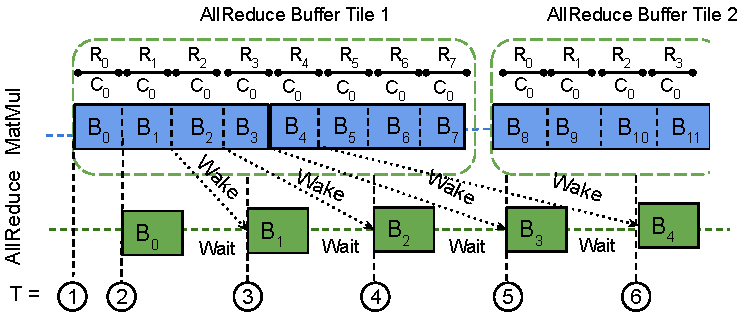
\includegraphics[width=\linewidth]{figures/overlap-example-rank-0.pdf}
% 		\caption{Workflow of overlap on \textbf{rank 0}. Rank 0 starts with chunks associated with Rank 0. }
% 	\end{subfigure}
	
% 	\begin{subfigure}{\linewidth}
% 		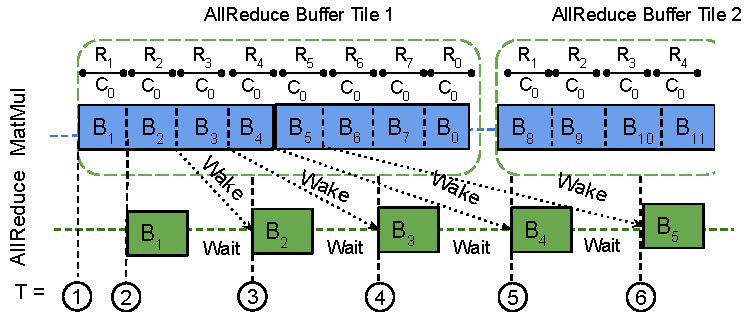
\includegraphics[width=\linewidth]{figures/overlap-example-rank-1.pdf}
% 		\caption{Workflow of overlap on \textbf{rank 1}. Rank 1 starts with chunks associated with Rank 1. }
% 	\end{subfigure}
% 	\caption{Workflow of \tool's overlapping of producer computation stage with a consumer \allreduce stage for data of size 128MB on 4 ranks (R$_0$ to R$_3$) with 2 channels (C$_0$ to C$_1$) and 64 MB buffer size. Size of each chunk is 8MB. \tool's custom communication kernel allows better overlapping without any decrease in communication bandwidth.
% 		\label{fig:workflow-overlap}}
% \end{figure*}

The example in Figure~\ref{fig:workflow-overlap} works as follows.
At T = \circled{1}, all ranks invoke MatMul and \allreduce kernels.
On rank 0, after computing chunk 0, the MatMul kernel wakes the \allreduce kernel at T = \circled{2}, which starts communicating chunk 0.
While on rank 1, at T = \circled{2} the MatMul kernel wakes the \allreduce kernel to communicate chunk 1.
%In parallel, the GEMM kernels on both ranks compute next chunks.
Concurrently, both MatMul kernels compute their corresponding next chunk.
At T = \circled{3}, MatMul kernels finished computing chunk 1 on rank 0 and chunk 2 on rank 1 and wakes up corresponding \allreduce kernels to communicate these chunks.
% Meanwhile, the GEMM kernel produces next chunks required by \allreduce.
This process continues until all chunks are processed.
%This process continues until the GEMM kernel finishes all chunks.

This process allows the MatMul kernel and \allreduce to be overlapped in a fine-grained manner,
which reduces the startup latency of \allreduce.
Since \allreduce communicates on the same chunk sizes, it achieves maximum communication bandwidth.
Furthermore, the MatMul kernel achieves maximum efficiency because the kernel is invoked on the full matrix size.
Figure~\ref{fig:matmul-overlap-intro} shows that this overlapping provides up to 1.36$\times$ better performance and hides more than 80\% of the MatMul time.

\subsection{Operations on Scattered Tensors}
\label{sec:scattered-tensors}
In data parallelism, communication and computation occur on different layers of widely different sizes.
Since machine learning frameworks allocate parameters and gradients of layers in non-contiguous buffers,
gradients are copied to a large buffer to avoid launching multiple \allreduce operations.
% The flatten and unflatten operations in Figure~\ref{fig:motivation} exemplify this problem.

\tool supports generating a single kernel for both computation and communication operations acting on non-contiguous tensors.
In this section, we show how \tool modifies NCCL to generate a single communication kernel for scattered tensors.
This code generation is non-trivial because NCCL has several design decisions based on the assumption that it is communicating a single contiguous buffer.
For example, each thread of a NCCL channel copies only a few elements in each iteration, and hence indexing the correct tensor at a particular offset requires a linear search through all non-contiguous tensors, which can lead to significant overhead.
\tool solves this problem by first dividing each tensor into buckets of size at most 2$^{10}$ elements and then assigning buckets to warps in a round-robin manner.
This mechanism allows each thread to quickly find the offset in a tensor, since a warp can directly index in its assigned bucket.
\tool pre-calculates the number of buckets that belong to the same contiguous buffer and calculates the offset for all of them once.

The process of breaking each tensor to buckets has computation overhead and extra memory requirements.
Since this bucketing is done only once on the CPU and training tasks run for thousands of iterations on the same tensors, the computation overhead is negligible.
Each bucket is represented by a pair of 64-bit tensor address and a 32-bit offset into the associated tensor, leading to $12 \times \left \lceil \frac{N}{2^{10}}\right \rceil$ bytes of extra memory for a tensor with $N$ elements.
However, this memory overhead is negligible for large models. For example, for BERT model with 334M elements, the memory requirement is 0.6\%.
Table~\ref{tab:scattered-tensors} shows that the overhead of scattered tensors is insignificant over contiguous tensors.

\begin{table}[t]
    \center
  \small
  \caption{Time to perform parameter update of all 360 tensors of BERT using Adam/LAMB on 256 Tesla V100 GPUs with scattered tensors implementation and a single contiguous tensor of size equal to the sum of size of all tensors.\label{tab:scattered-tensors}}
  \begin{tabular}{c|c|l}
  \textbf{Optimizer}   & \textbf{Scattered Tensor} & \textbf{Single Tensor}\\ \hline
  Adam & 33.89 ms & 33.21 ms  \\ 
  LAMB & 37.04 ms & 36.71 ms
  \end{tabular}
  \par \bigskip% Do not remove this. Without this there is no space between caption and the table
\end{table}

\subsection{PyTorch Integration}
\label{sec:pytorch-integration}
We integrated \tool generated code as a function to PyTorch's \texttt{torch.distributed} module.
This design allows us to re-use the logic for initializing NCCL and provide compatibility with models already using \texttt{torch.distributed}.
We added wrapper functions for calling \tool generated operations.
These wrapper functions prepare the arguments for calling \tool's operations, which includes pre-calculating pointers to the buckets for scattered tensors and clearing the spin-lock buffers for overlapping.
Machine learning models can invoke \tool functions using PyTorch.
\section{Experiments}
\label{sec:experiments}

We validate our approach empirically, showing that our Monarch matrix parametrization achieves a favorable efficiency--accuracy tradeoff compared to baselines on a wide range of domains (text, images, PDEs, MRI), in three settings (E2E training, S2D training, and D2S fine-tuning):
\begin{itemize}[leftmargin=*,nosep,nolistsep,noitemsep]
\item
In \cref{subsec:benchmark_tasks}, on image classification and language modeling benchmarks, such as ViT / MLP Mixer on ImageNet and GPT-2 on Wikitext-103, Monarch is 2$\times$ faster to train than dense models, while achieving the same accuracy / perplexity. In \cref{subsec:pde_mri}, in scientific and medical domains where special transforms (Fourier) are common, Monarch outperforms Fourier transform based methods on PDE solving, with up to 40\% lower error, and on MRI reconstruction attains up to 15\% higher pSNR and 3.8\% higher SSIM.
\item In \cref{subsec:pde_mri}, we show that on the large OpenWebText dataset, reverse sparsification (training with Monarch weight matrices for most of the time, then transitioning to dense weight matrices) speeds up the pretraining of GPT-2 models by 2$\times$ compared to the dense model, with no loss in upstream or downstream quality.
Moreover, reverse sparsification speeds up BERT pretraining by 23\% even compared to the implementation from Nvidia that set the MLPerf~\citep{mattson2020mlperf} 1.1 record.
\item In \cref{subsec:finetuning}, as a proof of concept, we demonstrate that our Monarch approximation algorithm can improve fine-tuning efficiency for pretrained models. We show that compressing BERT to a Monarch matrix model performs comparably to a finetuned dense model on GLUE, with 2$\times$ fewer parameters and 1.7$\times$ faster finetuning speed.
\end{itemize}

\subsection{End-to-End Training}
\label{subsec:e2e_training}
\subsubsection{Benchmark Tasks: Image Classification, Language Modeling}
\label{subsec:benchmark_tasks}

We show that replacing dense matrices with Monarch matrices in ViT, MLP-Mixer, and
GPT-2 can speed up training by up to 2$\times$ without sacrificing model quality in~\cref{table:pretrain,table:gpt_pretrain}.

\textbf{Setup.} We use the popular vision benchmark, ImageNet~\citep{deng2009imagenet}. We choose recent popular Vision Transformer~\citep{dosovitskiy2020image}, and MLP-Mixer~\citep{tolstikhin2021mlp} as representative base dense models.
For language modeling, we evaluate GPT-2~\citep{radford2019language} on WikiText-103~\citep{merity2016pointer}.

\begin{table}[h]
  \small
  \centering
  \vspace{-2mm}
  \caption{\label{table:pretrain}The performance of Monarch matrices and ViT / MLP-Mixer on ImageNet, including the number of parameters and FLOPs. We measure the Top-1 accuracy and the training time speedup compared to the corresponding dense model. %
  \vspace{2mm}
  }
  \iftoggle{arxiv}{}{
  \resizebox{\linewidth}{!}
  }
  {
  \setlength{\tabcolsep}{3pt}
  \vspace{3em}
  \begin{tabular}{@{}c||ccccccc@{}}
  \specialrule{.15em}{.05em}{.05em}
    Model&\multicolumn{1}{c}{ImageNet acc.}&\multicolumn{1}{c}{Speedup} &\multicolumn{1}{c}{Params} & \multicolumn{1}{c}{FLOPs} \\
    \specialrule{.15em}{.05em}{.05em}
    Mixer-S/16& 74.0& - & 18.5M & 3.8G \\
    Monarch-Mixer-S/16& 73.7& 1.7$\times$ & 7.0M & 1.5G \\
    Mixer-B/16& 77.7& - & 59.9M & 12.6G \\
    Monarch-Mixer-B/16& 77.8& 1.9$\times$ & 20.9M & 5.0G \\
    \specialrule{.15em}{.05em}{.05em}
    ViT-S/16& 79.4 & - & 48.8M & 9.9G \\
    Monarch-ViT-S/16& 79.1 & 1.9$\times$ & 19.6M & 3.9G \\
    ViT-B/16& 78.5 & - & 86.6M  & 17.6G \\
    Monarch-ViT-B/16& 78.9 & 2.0$\times$ & 33.0M & 5.9G \\
    \specialrule{.15em}{.05em}{.05em}
  \end{tabular}
  }
\end{table}

\begin{table}[h]
  \small
  \centering
  \vspace{-3mm}
  \caption{\label{table:gpt_pretrain} Performance of Monarch matrices and GPT-2-Small/Medium on WikiText-103, including the \# of parameters and FLOPs. Monarch achieves similar perplexity (ppl) but 2.0$\times$ faster.}
  \vspace{1mm}
  \iftoggle{arxiv}{}{
    \resizebox{0.95\linewidth}{!}
  }
  {
\setlength{\tabcolsep}{5pt}
\begin{tabular}{c||cccc}
\specialrule{.15em}{.05em}{.05em}
\multirow{1}{*}{{ Model} } & \multicolumn{1}{c}{\multirow{1}{*}{PPL}}
                              & \multicolumn{1}{c}{\multirow{1}{*}{Speedup}}
                              & \multicolumn{1}{c}{\multirow{1}{*}{Params}}
                              & \multicolumn{1}{c}{\multirow{1}{*}{FLOPs}}\\
\specialrule{.15em}{.05em}{.05em}
GPT-2-Small &  20.6 & - & 124M& 106G\\
Monarch-GPT-2-Small& 20.7  & 1.8$\times$ &72M & 51G\\
\specialrule{.15em}{.05em}{.05em}
GPT-2-Medium &  20.9 & - & 355M& 361G\\
Monarch-GPT-2-Medium& 20.3  & 2.0$\times$ &165M & 166G\\
\specialrule{.15em}{.05em}{.05em}
\end{tabular}
}
\vspace{-2mm}
\end{table}


\subsubsection{PDE solving and multi-coil MRI reconstruction}
\label{subsec:pde_mri}

Many scientific or medical imaging tasks rely on specialized transforms such as the
Fourier transform.
We show that replacing the fixed Fourier transform with the more expressive
Monarch matrices yields higher model quality (lower reconstruction error) with
comparable model speed.

\textbf{Solving PDEs with Monarch Neural Operators.}
We follow the experimental setting in FNO~\citep{li2020fourier} and apply a Monarch--based neural operator to the task of solving the Navier--Stokes PDE. Compared to baseline U-Nets~\citep{ronneberger2015u}, TF-Nets~\citep{wang2020towards}, ResNets~\citep{he2016deep} and FNOs~\cite{li2020fourier}, neural operators based on Monarch improve solution accuracy across spatial resolutions by up to $40\%$ (Table \ref{table:pde}).  





\paragraph{Non-periodic boundary conditions.} Traditional spectral methods based on Fourier transform work best with periodic boundary conditions and forcing terms. However, PDEs of practical interest often exhibit non--periodic or even unknown boundary conditions. Monarch operators are not constrained to the Fourier transform and can thus still learn the solution operator with excellent accuracy.

\begin{table}[h!] 
\scriptsize
\vspace{-4mm}
\caption{\label{table:pde}Benchmarks on Navier-Stokes (fixing resolution 64 × 64 for both training and testing).
Decreasing the viscosity coefficient $\nu$ makes the dynamics more chaotic.
}
\vspace{1mm}
\centering
\iftoggle{arxiv}{}{
  \resizebox{0.9\linewidth}{!}
}
{
\renewcommand{\arraystretch}{1}
\begin{tabular}{ c||ccc }
\specialrule{.15em}{.05em}{.05em}
Model & $v = 10^{-3}$  &  $v = 10^{-4}$ & $v = 10^{-5}$\\
\specialrule{.15em}{.05em}{.05em}
U-Net & 0.025  & 0.205  &   0.198\\
TF-Net  & 0.023  & 0.225 &  0.227 \\
ResNet & 0.070 &  0.287 &  0.275 \\
FNO & 0.017  & 0.178 & 0.155\\
Monarch-NO & \textbf{0.010} & \textbf{0.145} & \textbf{0.136} \\
\specialrule{.15em}{.05em}{.05em}
\end{tabular}
}
\textbf{\vspace{-3mm}}
\end{table}

\textbf{Accelerated MRI Reconstruction.} We characterize the utility of Monarch-based FFT operations for accelerated MRI reconstruction, a task which requires methods with both structured Fourier operators and dealiasing properties to recover high quality images. On the clinically-acquired 3D MRI SKM-TEA dataset \citep{desai2021skm}, Monarch-SENSE (mSENSE) enhances image quality by over 1.5dB pSNR and 2.5\% SSIM compared to zero-filled SENSE and up to 4.4dB and 3.8\% SSIM compared to U-Net baselines in data-limited settings. Setup details are available in~\cref{sec:experiment_details_mri}.

\paragraph{Expressive FFT.} By definition, standard IFFT in zero-filled SENSE cannot dealias the signal, resulting in artifacts in the reconstructed image. mSENSE replaces the inverse FFT (IFFT) operation in standard SENSE with learnable Monarch matrices. Thus, mSENSE preserves the structure of the Fourier transform while learning to reweight frequencies to suppress aliasing artifacts. Across multiple accelerations, mSENSE achieved up to +1.5dB and 2.5\% improvement in peak signal-to-noise ratio (pSNR) and structural similarity (SSIM), respectively (Table~\ref{table:mri}).

\paragraph{Data Efficiency.} While CNNs have shown promise for MRI reconstruction tasks, training these networks requires extensive amounts of labeled data to avoid overfitting. However, large data corpora are difficult to acquire in practice. mSENSE can be trained efficiently with limited supervised examples. In few shot settings, mSENSE can outperform U-Net by +4.4dB ($\approx$15\%) and 3.8\% SSIM (Table~\ref{table:mri-data-limited}). 







\begin{table}[h!] 
\scriptsize
\vspace{-3mm}
\caption{\label{table:mri}Mean $\pm$ standard error of the mean of conventional and Monarch-SENSE (mSENSE) on dual-echo (E1,E2) MRI reconstruction at multiple acceleration factors (Acc.).
}
\vspace{1mm}
\centering
\iftoggle{arxiv}{}{
  \resizebox{\linewidth}{!}
}
{
\renewcommand{\arraystretch}{1.2}
\begin{tabular}{c||ccccc}
\specialrule{.15em}{.05em}{.05em}
  & & \multicolumn{2}{c}{pSNR (dB) ($\uparrow$)} & \multicolumn{2}{c}{SSIM ($\uparrow$)} \\
  Acc. & Model &             E1 &             E2 &                E1 &                E2 \\
\specialrule{.15em}{.05em}{.05em}
\multirow{2}{*}{2} & SENSE &  32.8$\pm$0.2 &  35.4$\pm$0.2 &  0.871$\pm$0.003 &  0.865$\pm$0.003 \\
  & mSENSE &  \textbf{34.3$\pm$0.2} &  \textbf{36.6$\pm$0.2} &  \textbf{0.886$\pm$0.002} &  \textbf{0.882$\pm$0.003} \\
\specialrule{.15em}{.05em}{.05em}
\multirow{2}{*}{3} & SENSE &  30.9$\pm$0.2 &  33.5$\pm$0.2 &  0.819$\pm$0.004 &  0.795$\pm$0.004 \\
  & mSENSE &  \textbf{32.3$\pm$0.2} &  \textbf{34.6$\pm$0.2} &  \textbf{0.843$\pm$0.003} &  \textbf{0.820$\pm$0.004} \\
\specialrule{.15em}{.05em}{.05em}
\multirow{2}{*}{4} & SENSE &  30.1$\pm$0.2 &  32.8$\pm$0.2 &  0.789$\pm$0.004 &  0.753$\pm$0.005 \\
  & mSENSE &  \textbf{31.2$\pm$0.2} &  \textbf{33.5$\pm$0.2} &  \textbf{0.812$\pm$0.003} &  \textbf{0.767$\pm$0.005} \\
\specialrule{.15em}{.05em}{.05em}
\end{tabular}
}
\end{table}

\begin{table}[h!] 
\scriptsize
\vspace{-5mm}
\caption{\label{table:mri-data-limited}Impact of number of training examples ($N$) on dual-echo MRI reconstruction at 2x acceleration.
}
\vspace{1mm}
\centering
\iftoggle{arxiv}{}{
  \resizebox{\linewidth}{!}
}
{
\renewcommand{\arraystretch}{1.2}
\begin{tabular}{c||ccccc}
\specialrule{.15em}{.05em}{.05em}
  &  & \multicolumn{2}{c}{pSNR (dB) ($\uparrow$)} & \multicolumn{2}{c}{SSIM ($\uparrow$)} \\
  $N$ & Model &            E1 &            E2 &               E1 &               E2 \\
\specialrule{.15em}{.05em}{.05em}
N/A & SENSE &  32.8$\pm$0.2 &  35.4$\pm$0.2 &  0.871$\pm$0.003 &  0.865$\pm$0.003 \\
\specialrule{.15em}{.05em}{.05em}
\multirow{2}{*}{1} & U-Net &  29.4$\pm$0.2 &  34.4$\pm$0.3 &  0.848$\pm$0.004 &  0.857$\pm$0.004 \\
  & mSENSE &  \textbf{33.8$\pm$0.2} &  \textbf{36.0$\pm$0.2} &  \textbf{0.886$\pm$0.003} &  \textbf{0.867$\pm$0.003} \\
\specialrule{.15em}{.05em}{.05em}
\multirow{2}{*}{2} & U-Net &  29.9$\pm$0.3 &  35.1$\pm$0.3 &  0.858$\pm$0.003 &  0.871$\pm$0.003 \\
  & mSENSE &  \textbf{34.0$\pm$0.2} &  \textbf{36.4$\pm$0.2} &  \textbf{0.883$\pm$0.002} &  \textbf{0.877$\pm$0.003} \\
\specialrule{.15em}{.05em}{.05em}
\multirow{2}{*}{3} & U-Net &  31.0$\pm$0.3 &  35.2$\pm$0.3 &  0.866$\pm$0.003 &  0.867$\pm$0.004 \\
  & mSENSE &  \textbf{33.9$\pm$0.2} & \textbf{ 36.5$\pm$0.2} &  \textbf{0.882$\pm$0.002} & \textbf{0.878$\pm$0.003} \\
\specialrule{.15em}{.05em}{.05em}
\multirow{2}{*}{5} & U-Net &  31.4$\pm$0.3 &  35.6$\pm$0.2 &  0.877$\pm$0.002 &  0.870$\pm$0.003 \\
  & mSENSE &  \textbf{33.9$\pm$0.2} &  \textbf{36.5$\pm$0.2} &  \textbf{0.881$\pm$0.002} &  \textbf{0.877$\pm$0.003} \\
\specialrule{.15em}{.05em}{.05em}
\end{tabular}
}
\end{table}




\subsection{Sparse-to-Dense Training (reverse sparsification)}
\label{subsec:s2d_training}
\paragraph{GPT-2 pretraining.}
On the large OpenWebtext dataset~\citep{Gokaslan2019OpenWeb}, we train a GPT-2 model with Monarch weight
matrices for 90\% of the training iterations, then relax the constraint on the
weight matrices and train them as dense matrices for the remaining 10\% of the
iterations.
We call this technique ``reverse sparsification.''
Previous sparse training techniques often don't speed up training, whereas our
hardware-efficient Monarch matrices do.
Therefore we can use them as an intermediate step to pretrain a large language
model (GPT-2) in 2$\times$ less time. We also evaluate its downstream quality on zero-shot generation from~\citep{eval-harness} and classification tasks from~\citep{zhao2021calibrate}, achieving comparable performance to the dense counterparts (\cref{table:gpt_finetune}). 

\begin{table}[h]
  \small
  \centering
  \vspace{-3mm}
  \caption{\label{table:gpt_finetune}The performance (accuracy) of GPT-2-medium trained with Monarch reverse sparsification and with conventional dense training on text classification benchmarks.}
  \setlength{\tabcolsep}{5pt}
  \vspace{1em}
  \iftoggle{arxiv}{}{
    \resizebox{\linewidth}{!}
  }
  {
  \begin{tabular}{@{}c||ccc@{}}
    \specialrule{.15em}{.05em}{.05em}
    Model&\multicolumn{1}{c}{OpenWebText (ppl)}&\multicolumn{1}{c}{Speedup}& \multicolumn{1}{c}{Classification (avg acc)} \\
    \specialrule{.15em}{.05em}{.05em}
    GPT-2m& 18.0 & - & 38.9 \\
    Monarch-GPT-2m& 18.0 & 2$\times$ & 38.8 \\
    \specialrule{.15em}{.05em}{.05em}
  \end{tabular}
  }
  \vspace{-3mm}
\end{table}


In \cref{fig:reverse_sparsification_bar}, we show the training time of the dense GPT-2 model, along with
the Monarch GPT-2 model.
After training the Monarch model for 90\% of the time, in the
last 10\% of the training steps, by transitioning to dense weight matrices, the model is able to reach the same 
performance of another model that was trained with dense weight matrices from
scratch.
By training with Monarch matrices for 90\% of the time, we reduce the total training time by 2$\times$.

\paragraph{BERT pretraining.}
On the Wikipedia + BookCorpus datasets~\citep{zhu2015aligning}, we train a BERT-large model with Monarch weight matrices for 70\% of the time and transition to dense weight matrices for the remaining 30\% of the time, which yields the same pretraining loss as conventional dense training.
In \cref{table:bert_speed}, we compare the total training time to several baseline implementations: the widely-used implementation from HuggingFace~\citep{wolf-etal-2020-transformers}, the more optimized implementation from Megatron~\citep{shoeybi2019megatron}, and the most optimized implementation we know of from Nvidia that was used to set MLPerf 1.1 training speed record. Our method is 3.5x faster than HuggingFace and 23\% faster than Nvidia's MLPerf 1.1 implementation\footnote{Our result is not an official MLPerf submission. We train BERT for both phase 1 (sequence length 128) and phase 2 (sequence length 512) according to the standard BERT training recipe\cite{devlin2018bert}, while MLPerf only measures training time for phase 2.}.
Experiment details are in~\cref{subsec:bert_details}.

\begin{table}[h]
  \small
  \centering
  \caption{\label{table:bert_speed}The total training time of BERT-large trained with Monarch reverse sparsification and with conventional dense training on 8 A100-40GB GPUs (DGX A100). Training consists of two phases, phase 1 with sequence length 128 and phase 2 with sequence length 512. Monarch training is 3.5x faster than HuggingFace and 23\% faster than Nvidia's MLPerf 1.1 implementation.}
  \vspace{1em}
  \iftoggle{arxiv}{}{
    \resizebox{\linewidth}{!}
  }
  {
    \begin{tabular}{@{}c||c@{}}
      Implementation & Training time (h)  \\ \hline
      HuggingFace &  84.5 \\
      MegaTron & 52.5 \\
      Nvidia MLPerf 1.1 & 30.2 \\
      Nvidia MLPerf 1.1 + DeepSpeed & 29.3 \\
      Monarch (ours) & \textbf{23.8} \\
    \end{tabular}
  }
  \vspace{-3mm}
\end{table}

\subsection{Dense-to-Sparse Fine-tuning}
\label{subsec:finetuning}

\begin{figure}[t]
  \centering
  \vspace{-3mm}
  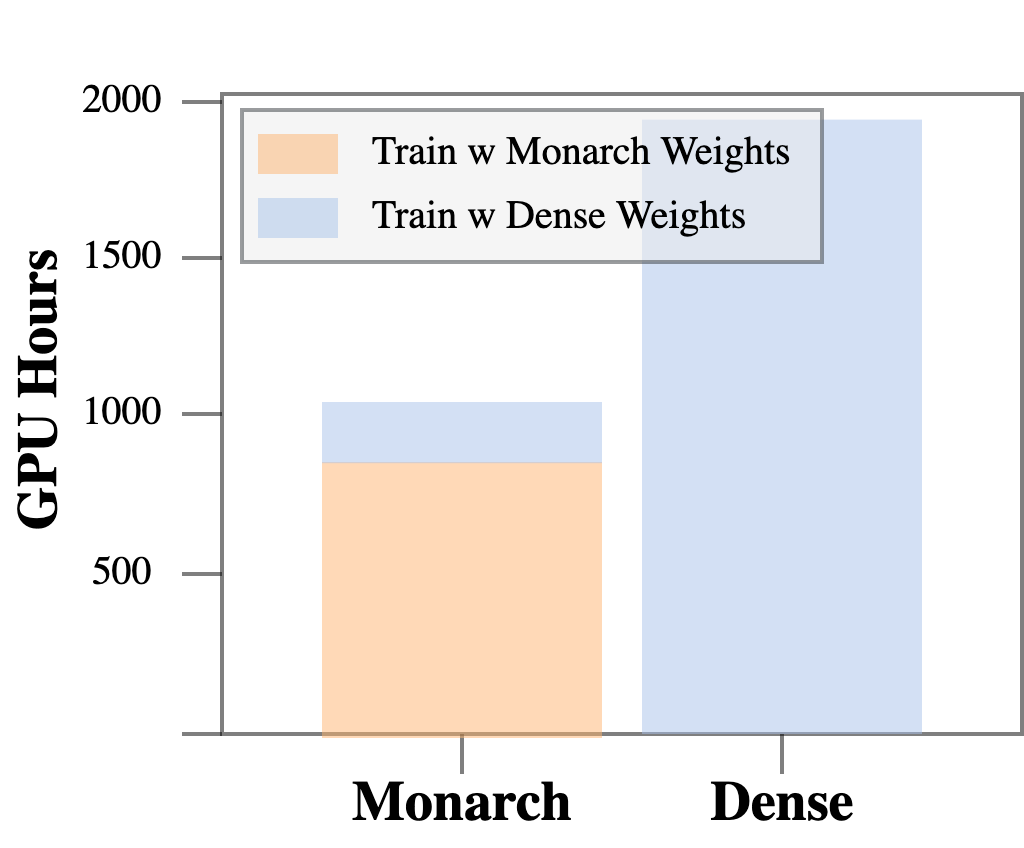
\includegraphics[width=.3\textwidth]{figures/rv_bar_temp.png}
  \vspace{-3mm}
  \caption{\label{fig:reverse_sparsification_bar}Time required (in A100 GPU hours) to reach the same perplexity (18.0)
    for GPT-2-small on OpenWebText.
    With ``reverse sparsification'', Monarch can speed up
    GPT-2 training by 2$\times$.\vspace{-1em}}
\end{figure}

We show that our Monarch approximation algorithm allows us to efficiently use
pretrained models, such as speeding up BERT finetuning on GLUE.

\paragraph{BERT finetuning.}
We take the BERT pretrained weights, approximate them with Monarch matrices,
and finetune the resulting model on the 9 GLUE tasks.
The results in \cref{table:bert_glue} shows that we obtain a Monarch finetuned
model with similar quality to the dense BERT model, but with 1.7$\times$ faster
finetuning speed.
This serves as a proof of concept, and we expect further speedup if additional model compression techniques are applied (e.g., quantization, kernel fusion).




\begin{table}[h]
  \small
  \centering
  \vspace{-5mm}
  \caption{\label{table:bert_glue}The performance of Monarch matrices in
    finetuning BERT on GLUE.}
  \setlength{\tabcolsep}{5pt}
  \vspace{1em}
  \iftoggle{arxiv}{}{
    \resizebox{\linewidth}{!}
  }
  {
  \begin{tabular}{@{}c||ccccccc@{}}
  \specialrule{.15em}{.05em}{.05em}
    Model&\multicolumn{1}{c}{GLUE (avg)}&\multicolumn{1}{c}{Speedup} &\multicolumn{1}{c}{Params} & \multicolumn{1}{c}{FLOPs} \\
    \specialrule{.15em}{.05em}{.05em}
    BERT-base & 78.6& - & 109M & 11.2G \\
    Monarch-BERT-base& 78.3& 1.5$\times$ & 55M & 6.2G  \\
    BERT-large & 80.4 & - & 335M & 39.5G \\
    Monarch-BERT-large & 79.6 & 1.7$\times$ & 144M & 14.6G  \\
    \specialrule{.15em}{.05em}{.05em}
  \end{tabular}
  }
  \vspace{-3mm}
\end{table}



%!TEX root = ../main.tex

\section{Related Work}
\label{sec:related}

\textbf{State space models} have shown promise in modeling sequential data, including time series data~\citep{gu2022efficiently}, audio~\citep{goel2022s}, and visual data~\citep{nguyen2022s4nd}.
Our model builds off work on simplifying and parameterizing diagonal versions of S4~\citep{gu2022parameterization,gupta2022diagonal, gu2022train}.
Gated state spaces~\citep{mehta2022long} also aim to adapt SSMs to language modeling, but our results suggest that the GSS model does not perform as well as \hthree (or even as well as earlier SSMs like S4D).
The idea to combine SSMs with attention in hybrid models is not new; Mehta et al.~\citep{mehta2022long} also showed that interleaving attention with their GSS layer can improve performance, which we also validate on our OpenWebText experiments.
These positive results suggest that attention and SSMs are complementary, and that hybrid models may be a promising direction for future work.

\textbf{Large language foundation models}~\citep{bommasani2021opportunities} have demonstrated the power of scaling attention-based networks to billions of parameters and training them on trillions of tokens~\citep{hoffmann2022training}.
Understanding the mechanistic basis~\citep{elhage2021mathematical} behind these models may yield insights into better design choices for future models.
These and similar explorations have informed the design of \hthree and our selection of synthetic languages.
A number of recent works have also explored how to address the shortcomings of attention by approximating the attention computation~\citep{wang2020linformer,katharopoulos2020transformers, choromanski2020rethinking,tay2020long, kitaev2020reformer, daras2020smyrf}.
We believe these efforts are complementary to SSMs, and we are excited to see how they can be combined in future work.

\textbf{Linear attention}~\citep{katharopoulos2020transformers} and classical sequence models like RNNs serve as inspiration for \hthree.
Appendix~\ref{app:linear_attention} draws a direct connection between linear attention and LTI systems.
Luo et al.~\citep{luo2021stable} also propose a variant of linear attention that can achieve $O(n \log n)$ scaling in sequence length.
Appendix~\ref{sec:app_additional_experiments} evaluates linear attention on language modeling, and finds that it underperforms exact attention, whereas \hthree outperforms attention.
The multiplicative interactions in \hthree are reminiscent of gating mechanisms in LSTMs~\citep{hochreiter1996lstm} and GRUs~\citep{cho2014properties}, which suggests that architectural lessons from these sequence models may be useful for adapting SSMs to language modeling.
A number of algorithms for scaling attention to longer sequences have also been proposed, such as Transformer-XL~\citep{dai2019transformer}, Reformer~\citep{kitaev2020reformer}, Performer~\citep{choromanski2020rethinking}, and Perceiver AR~\citep{hawthorne2022general}.
Some of these approaches underperform exact attention on language modeling, and may be slower in wall-clock speed~\citep{dao2022flashattention}.
A thorough comparison of these alternatives to exact attention and how well they scale in model size and amount of training data is fruitful future work.

\textbf{FFT} algorithms are used in a wide variety of applications, including signal processing~\citep{oppenheim1978applications}, control theory~\citep{brogan1974modern}, and more.
Various algorithms for computing the FFT have existed for decades~\citep{oppenheim2001discrete}.
We hope our work on appealing to these classic algorithms to accelerate new applications such as learned SSMs will inspire future algorithmic exploration, even if hardware is not designed for them~\citep{hooker2021hardware}.

%%% Local Variables:
%%% mode: latex
%%% TeX-master: "../main"
%%% End:


Hyperbolic embeddings embed hierarchical information with high
fidelity and few dimensions. We explored the limits of this approach
by describing scalable, high quality algorithms. We hope the
techniques here encourage more follow-on work on the exciting
techniques of \citet{fb, ucl}. As future work, we hope to explore how
hyperbolic embeddings can be most effectively incorporated into downstream
tasks and applications.

\section{Data Availability Statement}
The artifact for this paper~\cite{coconet-artifact} contains the source code of our implementation of \tool and the benchmarking infrastructure to reproduce all the results in Section~\ref{sec:experiments}.

\begin{acks}
We thank the reviewers and our shepherd, Tyler Sorensen, for their constructive feedback.
This work was partially supported by the National Science Foundation grant CCF-2052696.
\end{acks}


\appendix
\section{Artifact Appendix}

%%%%%%%%%%%%%%%%%%%%%%%%%%%%%%%%%%%%%%%%%%%%%%%%%%%%%%%%%%%%%%%%%%%%%
\subsection{Abstract}

This artifact appendix describes how to reproduce results for
standalone experiments in Figure~\ref{fig:bandwidth64GPUs},
~\ref{fig:matmul-overlap}, and ~\ref{fig:pipeline-overlap} and integration 
results in Section~\ref{sec:experiments:bert},~\ref{sec:experiments:model-parallel:integeration}, and ~\ref{sec:experiments:pipeline-parallel:integeration}.
This artifact includes the \tool{} DSL and compiler, and \tool{}'s generated code integrated 
with PyTorch, Megatron-LM, and NVIDIA Bert.
To reproduce the results, the experiments should be executed on a system similar to our experimental system.
However, all experiments can be executed on a system with more than one NVIDIA GPUs.

\subsection{Artifact Check-list (Meta-information)}

{\small
\begin{itemize}
  \item {\bf Program:} \tool{} DSL and compiler written in C++.
  \item {\bf Compilation:} A C++ compiler (\texttt{g++} or \texttt{clang}) to compile \tool{}. A C++ compiler with MPI support (\texttt{mpicxx}) and CUDA compiler (\texttt{nvcc}) to compile generated programs.
  \item {\bf Binary:} Each \tool{} program compiles to a binary that generates an MPI program containing CUDA kernels.
  \item {\bf Data set:} BERT, GPT-2, and GPT-3 training datasets for integration experiments. 
  % We provide instructions to download datasets.
  \item {\bf Run-time environment:} Ubuntu 20.04 with Python 3.7+, CUDA 11.0+, and OpenMPI 4.0+.
  \item {\bf Hardware:} We performed experiments on 16 NVIDIA DGX-2 nodes, i.e., a total of 256 NVIDIA Tesla V100 GPUs. 
  However, the experiments can be executed on any system with two or more GPUs.
  % The functionality of standalone experiments (Figure~\ref{fig:bandwidth64GPUs},~\ref{fig:matmul-overlap}, and ~\ref{fig:pipeline-overlap}) can be tested with as low as 2 GPUs, however, the integration experiments (Section~\ref{sec:experiments:bert},~\ref{sec:experiments:model-parallel:integeration}, and ~\ref{sec:experiments:pipeline-parallel:integeration}) requires atleast 16 DGX-2 nodes to run.
  \item {\bf Run-time state:} Python, MPI, and CUDA.
  \item {\bf Execution:} Use \texttt{mpirun} to run the experiments.
  \item {\bf Metrics:} Decrease in execution time of benchmarks.
  \item {\bf Output:} Execution time of each experiment and \tool{} speedup over baselines.
  \item {\bf Experiments:} Execution of standalone experiments and training and inference tasks of BERT, GPT-2, and GPT-3 models.
  \item {\bf How much disk space required (approximately)?:} 100 GB in total. 90\% of the space usage is required for storing dataset.
  \item {\bf How much time will be spent in preparing the workflow (approximately)?:} 1 hour.
  \item {\bf How much time is needed to complete experiments (approximately)?:} 5 hours.
  \item {\bf Publicly available?:} Yes.
\end{itemize}
}

%%%%%%%%%%%%%%%%%%%%%%%%%%%%%%%%%%%%%%%%%%%%%%%%%%%%%%%%%%%%%%%%%%%%%
\subsection{Description}

\subsubsection{How to Access}

The \tool{} implementation and the benchmarking infrastructure used in our evaluation are publicly available as the artifact~\cite{coconet-artifact}. 
This artifact contains a zip file with two directories: (i) \texttt{coconet}, which is the implementation of \tool{}, and (ii) \texttt{coconet-experiments}, which is the benchmarking infrastructure.
Latest versions of these directories are available at \url{https://github.com/parasailteam/coconet} and \url{https://github.com/parasailteam/coconet-experiments}.

\subsubsection{Hardware Dependencies}
All benchmarks can be executed on a distributed system with two or more NVIDIA GPUs.
However, our results will be reproducible on the evaluation system described in Section~\ref{sec:experiments}.

\subsubsection{Software Dependencies}
Our experiments require a system running Ubuntu 20.04 with Python 3.8+ and CUDA 11.0+.
Prerequisites and their installation procedure is described in \texttt{README.md} files of \texttt{coconet} and \texttt{coconet-experiments} directories.

\subsubsection{Data Sets}
The standalone benchmarks (Figure~\ref{fig:bandwidth64GPUs},~\ref{fig:matmul-overlap}, and ~\ref{fig:pipeline-overlap}) do not require any dataset.
Datasets required for executing experiments in Section~\ref{sec:experiments:bert},~\ref{sec:experiments:model-parallel:integeration}, and ~\ref{sec:experiments:pipeline-parallel:integeration} can be obtained by following \textit{Dataset} section of \texttt{README.md} in \texttt{coconet-experiments}.
%%%%%%%%%%%%%%%%%%%%%%%%%%%%%%%%%%%%%%%%%%%%%%%%%%%%%%%%%%%%%%%%%%%%%
\subsection{Installation}
Following instructions have been tested with Ubuntu 20.04.

\paragraph{Standalone Experiments Dependencies} Install dependencies by following the \textit{Prerequisites} section in \texttt{README.md} file of \texttt{coconet} directory.

\paragraph{Integration Experiments Dependencies} Follow the \textit{Prerequisites} section in \texttt{README.md} file of \texttt{coconet-experiments} directory to build PyTorch and install all dependencies for Megatron-LM and NVIDIA Bert.

%%%%%%%%%%%%%%%%%%%%%%%%%%%%%%%%%%%%%%%%%%%%%%%%%%%%%%%%%%%%%%%%%%%%%
\subsection{Experiment Workflow}
\subsubsection{Standalone Experiments}
\label{appendix:sec-standalone}
This section describe how to execute standalone experiments of Section~\ref{sec:experiments} and produce results for Figure~\ref{fig:bandwidth64GPUs}, Figure~\ref{fig:matmul-overlap}, and Figure~\ref{fig:pipeline-overlap}.
All of these experiments will take 1 hour combined.
\begin{enumerate}
  \item Install all \tool prerequisites in \texttt{coconet/README.md}.
  \item The \texttt{experiments/} directory contains all scripts for standalone experiments.

{\footnotesize
\begin{lstlisting}[language=bash]
$ cd coconet/experiments/
\end{lstlisting}
}

  \item Since all our experiments uses MPI to run the executable on all GPUs,  set the environment variable \texttt{NPROC} to the number of GPUs in the system. In our experiments, we set \texttt{NPROC} to 256 as follows:
  
  {\footnotesize
\begin{lstlisting}[language=bash]
$ export NPROC=256
\end{lstlisting}
}
\textbf{Note}: Setting \texttt{NPROC} to a value more than the number of GPUs in a system can lead to failed experiments.

  \item If the experiments are performed on a system with multiple nodes then additional arguments to \texttt{mpirun} can be passed by setting the \texttt{MPI\_ARGS} environment variable.
\end{enumerate}

\paragraph{Data-Parallel Experiments}
\begin{enumerate}
  \item To execute standalone data parallel experiments execute \texttt{data-parallel-exp.py}. This script takes a directory to store the results as an argument.
  Additionally, the script requires \texttt{MASTER\_ADDR} and \texttt{MASTER\_PORT} to be passed as \texttt{MPI\_RUN\_ARGS}. If the experiments are done on a single system, then it is common to set \texttt{MASTER\_ADDR=127.0.0.1} and \texttt{MASTER\_PORT=10000}.

  {\footnotesize
\begin{lstlisting}[language=bash]
$ export MPI_ARGS="-x MASTER_ADDR=127.0.0.1"
$ export MPI_ARGS="$MPI_ARGS -x MASTER_PORT=10000"
$ python data-parallel-exp.py results/
\end{lstlisting}
}

  The above execution of script will execute all data parallel executables and store the results in the \texttt{results} directory.

  \item Generate both graphs of Figure~\ref{fig:bandwidth64GPUs} by executing the script \texttt{gen-data-parallel-graphs.py}. This script takes the directory with results generated in the previous step as an argument.
  
{\footnotesize
\begin{lstlisting}[language=bash]
$ python gen-data-parallel-graphs.py results/
\end{lstlisting}
}

Graphs are stored in two files of \texttt{experiments} directory: \texttt{results-adam-fp16.pdf} and \texttt{results-lamb-fp16.pdf}.
\end{enumerate}

\paragraph{Model-Parallel Experiments}
\begin{enumerate}
  \item To execute standalone model-parallel experiments execute \texttt{model-parallel-exp.py}. Similar to the previous script, this script also takes a directory to store results as its argument.
  
  {\footnotesize
\begin{lstlisting}[language=bash]
$ python model-parallel-exp.py results/
\end{lstlisting}
}

  The script will execute all model parallel executables and stores the results in the \texttt{results} directory.
  \item Generate Figure~\ref{fig:matmul-overlap} by executing following script. This script will take above results directory as its argument. 
  
{\footnotesize
\begin{lstlisting}[language=bash]
$ python gen-model-parallel-graphs.py results/
\end{lstlisting}
}

Graph is stored as \texttt{results-model-parallel.pdf}.
\end{enumerate}

\paragraph{Pipeline-Parallel Experiments}
\begin{enumerate}
  \item To execute standalone pipeline-parallel experiments execute \texttt{pipeline-parallel-exp.py}. This script also requires a directory to store results as its command line argument.

  {\footnotesize
\begin{lstlisting}[language=bash]
$ python pipeline-parallel-exp.py results/
\end{lstlisting}
}

  Above execution of the script will execute all pipeline parallel executables and store the results in \texttt{results} directory.
  \item To generate Figure~\ref{fig:pipeline-overlap} execute the script \\ \texttt{gen-pipeline-parallel-graphs.py}. This script takes the directory containing above results as its argument.
  
{\footnotesize
\begin{lstlisting}[language=bash]
$ python gen-pipeline-parallel-graphs.py results/
\end{lstlisting}
}

The graph is stored in \texttt{results-model-parallel.pdf}.
\end{enumerate}

\subsubsection{Integration Experiments}
\label{appendix:sec-integration}
In this section, we will execute the integration experiments of Section~\ref{sec:experiments:bert},~\ref{sec:experiments:model-parallel:integeration}, and~\ref{sec:experiments:pipeline-parallel:integeration}.

\paragraph{Prerequisites} Install prerequisites and obtain dataset by following the steps in \texttt{coconet-experiments/README.md}.

\paragraph{Data-Parallel Training}
Go to \texttt{Nvidia-Bert} directory and execute \texttt{coconet-experiments.py}.

{\footnotesize
\begin{lstlisting}[language=bash]
$ cd NV-BERT 
$ python coconet-experiments.py
\end{lstlisting}
}

This script will execute data parallel training experiments and then print Table~\ref{tab:bert-results}.
This experiment will take 1 hour to complete.
This script contains maximum batch sizes supported by each implementation for our evaluation system of 256 Tesla V100 GPUs.
It is possible that for a different system the maximum batch size will be different.
The batch size dictionary in \texttt{coconet-experiments.py} can be modified to find maximum batch size for underlying system.

\paragraph{Model-Parallel Inference} 
Go to \texttt{MegatronLM-Model-Parallel} directory and execute \texttt{coconet-experiments.py}.
{\footnotesize
\begin{lstlisting}[language=bash]
$ cd MegatronLM-Model-Parallel
$ python coconet-experiments.py
\end{lstlisting}
}
This script will execute model parallel inference experiments and then print the values in Section~\ref{sec:experiments:model-parallel:integeration}.
This experiment will take less than 30 minutes to complete.

\paragraph{Pipeline-Parallel Inference} 
Execute \texttt{coconet-experiments.py} in the directory
\texttt{MegatronLM-Pipeline-Parallel}.
{\footnotesize
\begin{lstlisting}[language=bash]
$ cd MegatronLM-Pipeline-Parallel
$ python coconet-experiments.py
\end{lstlisting}
}
This script will execute pipeline parallel inference experiments and then print the table in Section~\ref{sec:experiments:pipeline-parallel:integeration}.
This experiment will take 3 hour to complete.
%%%%%%%%%%%%%%%%%%%%%%%%%%%%%%%%%%%%%%%%%%%%%%%%%%%%%%%%%%%%%%%%%%%%%
\subsection{Evaluation and Expected Results}

\paragraph{Standalone Experiments} The figures generated by the experiments of Section~\ref{appendix:sec-standalone} can be matched with the figures: \ref{fig:bandwidth64GPUs}, \ref{fig:matmul-overlap}, and \ref{fig:pipeline-overlap}.

\paragraph{Integration Experiments}
The results generated in experiments of Section~\ref{appendix:sec-integration} can be matched with the results in Section~\ref{sec:experiments:bert},~\ref{sec:experiments:model-parallel:integeration}, and~\ref{sec:experiments:pipeline-parallel:integeration}.

%%%%%%%%%%%%%%%%%%%%%%%%%%%%%%%%%%%%%%%%%%%%%%%%%%%%%%%%%%%%%%%%%%%%%
% \subsection{Methodology}

% Submission, reviewing and badging methodology:

% \begin{itemize}
%   \item \url{https://www.acm.org/publications/policies/artifact-review-badging}
%   \item \url{http://cTuning.org/ae/submission-20201122.html}
%   \item \url{http://cTuning.org/ae/reviewing-20201122.html}
% \end{itemize}

\balance
%-------------------------------------------------------------------------------
\bibliographystyle{ACM-Reference-Format}
\interlinepenalty=10000
\bibliography{paper}

%%%%%%%%%%%%%%%%%%%%%%%%%%%%%%%%%%%%%%%%%%%%%%%%%%%%%%%%%%%%%%%%%%%%%%%%%%%%%%%%
\end{document}
%%%%%%%%%%%%%%%%%%%%%%%%%%%%%%%%%%%%%%%%%%%%%%%%%%%%%%%%%%%%%%%%%%%%%%%%%%%%%%%%

%%  LocalWords:  endnotes includegraphics fread ptr nobj noindent
%%  LocalWords:  pdflatex acks
